

%% I need to describe muon ID in chaper 4.2 and Tau decay mode finding, tau MVA ID around 4.2 too 
\chapter{LFV event selection}
In both 8 TeV $H\rightarrow e\tau_h$ and 13 TeV $H\rightarrow\mu\tau_h$ analyses, events are selected in several steps. A loose selection selects on the different IDs, energy, geometry parameters of the analysis related objects. In the $\mcol$ fit analysis this is followed by a tighter set of selection criteria in which selection requirements are placed on the kinematics variables and fits on variable $\mcol$ in both  $H\rightarrow e\tau_h$ and $H\rightarrow\mu\tau_h$ analysis. This selection sequence is referred as $\mcol$ fit analysis. In $H\rightarrow\mu\tau_h$, there is an alternate selection sequence that follows the loose selection. A multivariate analysis with a Boosted decision tree (BDT) is defined and fits on the BDT discriminator. This is referred as the BDT fit analysis and provides more sensitive results in $\Hmuhad$ analysis. 



\section{\texorpdfstring{$H\rightarrow\mu\tau_h$}{Lg}}
\subsection{Loose selection}
Tau leptons from signal events decay hadronically. A SM Higgs boson is much heavier than its decay products $\mu$ and $\tau$. The $\mu$ and $\tau$ leptons are expected to have high $P_{T}$. As the decay products from signal events are boosted, therefore a cut on $\Delta R=\sqrt(\Delta phi^{2}+\Delta eta^{2})$, $\Delta R>0.3$ is applied. The $\mu$ and $\tau$ candidates are required to have opposite sign of charge as the Higgs boson is neutral. Further, events with additional $\mu$ and $\tau$ that pass the loose selection and events with jets that are identified by the combined secondary vertex(CSVv2) b-tagging algorithm \cite{btag_ago} as a b quark jets are vetoed. The trigger HLT\_IsoMu24 or HLT\_IsoTkMu24 used in the analysis selects isolated muons that have energy higher than 24 GeV at HLT level. A further $P_{T}$ cut on the reconstructed $\mu$,  $P_{T}>26$ GeV and $|\eta|<2.4$ are required. Muons are required to pass the recommended Medium muon ID and tight cut based isolation $I^{\mu}_{rel}<0.15$. %For the LHC data 2016, running period BCDEF, ICHEP medium muon ID is applied(table~\ref{tbl:ICHEPMedID}), for data running period G and H, also the monte Carlo samples, standard medium muon ID(table~\ref{tbl:standardMedID})are applied to achieve the best performance for muon identification.

Hadronic taus are required to have $P_T>30$ GeV,$|\eta|<2.3$, passing old tau decay mode finding, the MVA based tight tau isolation ID and tau discriminators against electrons and muons. %The discriminators are very loose MVA based rejection against electrons and cut-based tight rejection against muons.  


Events in the analysis are divided into four categories based on the number of jets. In 2-jets category, it is furthered divided into 2 categories,  2-jet gluon gluon fusion higgs production(ggH) category and 2-jet vector boson fusion(VBF) category based on the value of 2 jets invariant mass($M_{jj}$) . The 0-jet category enhances ggH production mode. In 1-jet category, the dominant signal production mode is also ggH, but with a boosted jet associated with the production and VBF higgs production also contributes this category. In the 2-jet ggH category, signal events mainly come from ggH, while in 2-jet VBF, VBF higgs is the dominant production channel.  The following is a more detailed list of the selection condition in each categories.

\begin{enumerate}
\item[{\bf 0-jet:}] No events have jets pass the loose PF ID and  with jet $P_T>30$ GeV, $|\eta|<4.7$.
\item[{\bf 1-jet:}] Events with one jet passes losse PF ID and jet $P_T>30$ GeV, $|\eta|<4.7$.
\item [{\bf 2-jets ggH:}] Events have two jets passing loose PF ID, $P_T>30$ GeV, $|\eta|<4.7$ and a requirement on the invariant mass of the two jets, $\textrm{M}_{jj}<550$ GeV. 
\item [{\bf 2 jets VBF:}] Events with two jets pass loose PF ID. Jets $P_T>30$ GeV, $|\eta|<4.7$ and $\textrm{M}_{jj}>550$ GeV are required. 
\end{enumerate} The threshold on $\textrm{M}_{jj}$ has been optimized to give the best expected exclusion limits.


\subsection{Cut-based analysis}
After the loose selection and the categorization, a further cut-based selection is applied. Variables that can help distinguish signal from background are $P_{T}^{\mu}$, $P_{T}^{\tau}$ and $M_{T}(\tau_{h})$. The lepton $P_{T}$ variables are very powerful background discriminant variables, but will also cause the problem that signal peaks under backgrounds. As leptons from signal process  tend to have higher $P_{T}$ values, cutting tighter on the lepton $P_{T}$, removes more background events. However this will also reshape some of the backgrounds, making them peak closer under the signal so that signal processes will be affected more by the background statistics fluctuation. In the $H\rightarrow e\tau_h$ analysis, the effect of cutting tighter on lepton $P_{T}$ will be shown. In $H\rightarrow\mu\tau_h$ search, lepton $P_{T}$ variables are kept at loose values and optimized on other variables to achieve tighter expected limits. 

The optimization is procedure uses only Monte Carlo samples so as not to double use data. In $\Hmuhad$  channel, the variables tuned are $\textrm{M}_{jj}$ and $M_{T}(\tau_{h})$. The selection criteria has been optimized to have the most stringent expected limits with the Asimov dataset(background only). The name Asimov dataset is inspired by the short story Franchise, by Isaac Asimov. If looser values of the cuts give the same expected limits as the tighter ones, then the looser cut values are chosen to have more statistics. Examples of optimization by checking the limits are shown in Figure. \ref{fig:optMT} and~\ref{fig:optVBFmass}, in which the optimization of $M_T(\tau_{h})$  and $\textrm{M}_{jj}$ are shown. A full summary of the cuts optimized for $\Hmuhad$ is shown in Table.~\ref{tab:Mhadcategories}


\begin{figure}[htbp] 
     \centering
     \subfigure[0 jet]{ 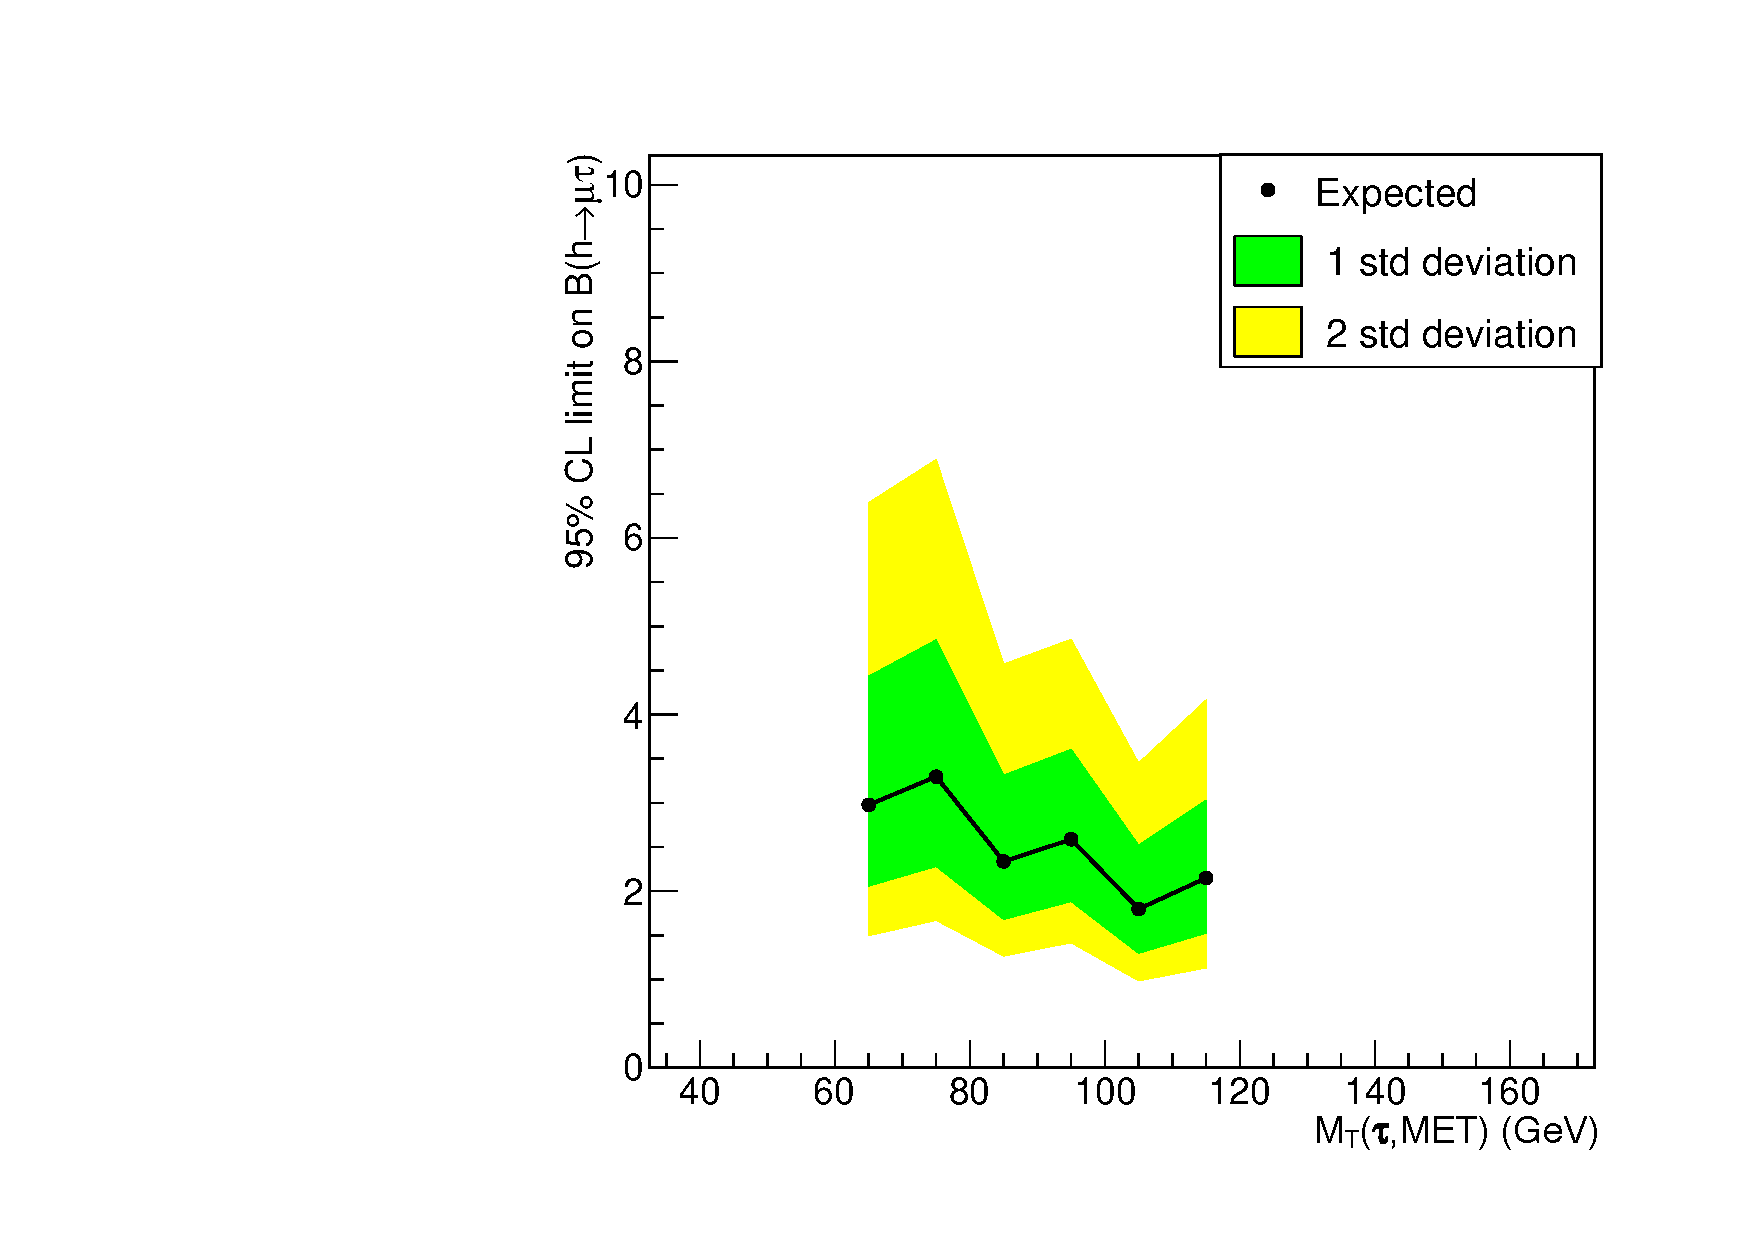
\includegraphics[width=0.4\textwidth]{chapter5/Tuning/ggtMtToPfMet_type1.pdf}}
     \subfigure[1 jet]{ 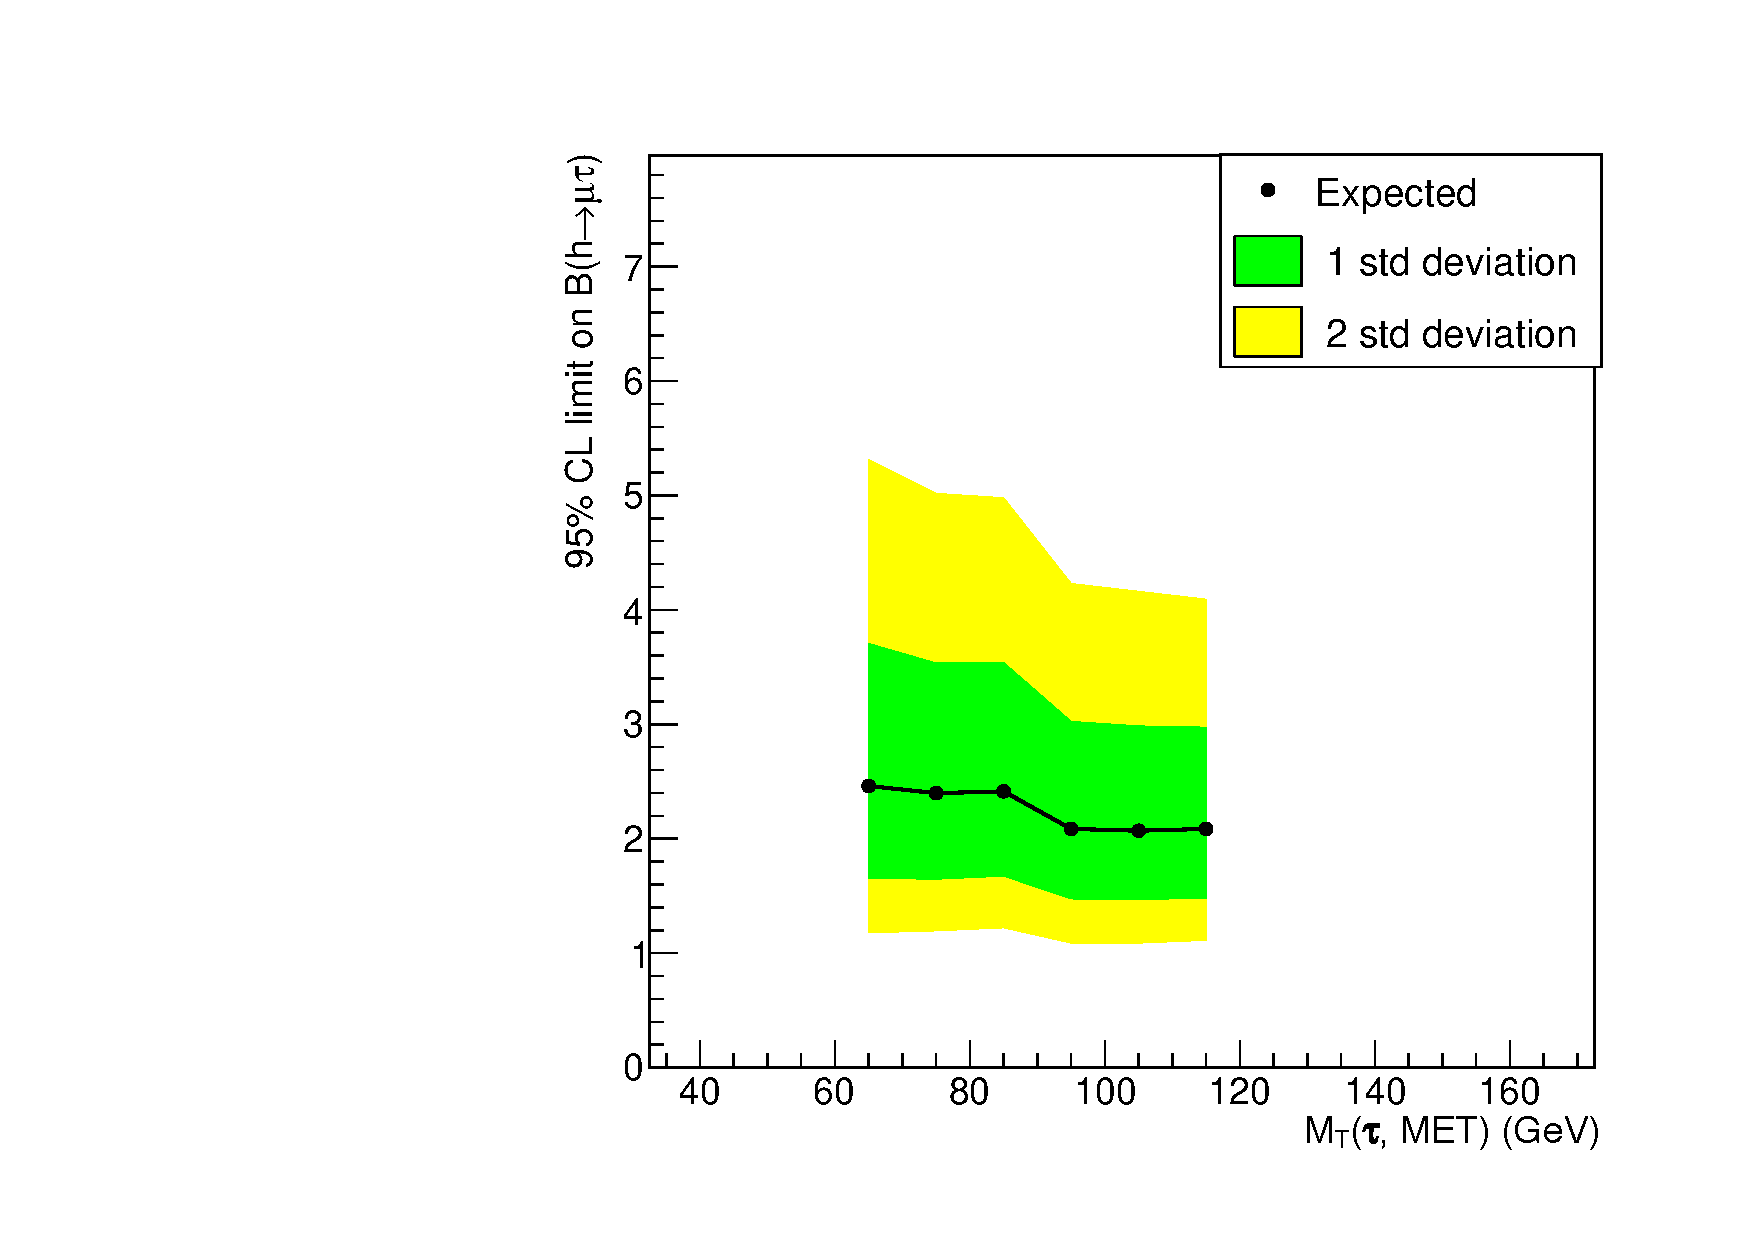
\includegraphics[width=0.4\textwidth]{chapter5/Tuning/boosttMtToPfMet_type1.pdf}}\\
     \subfigure[2 jets, gg-enriched]{ 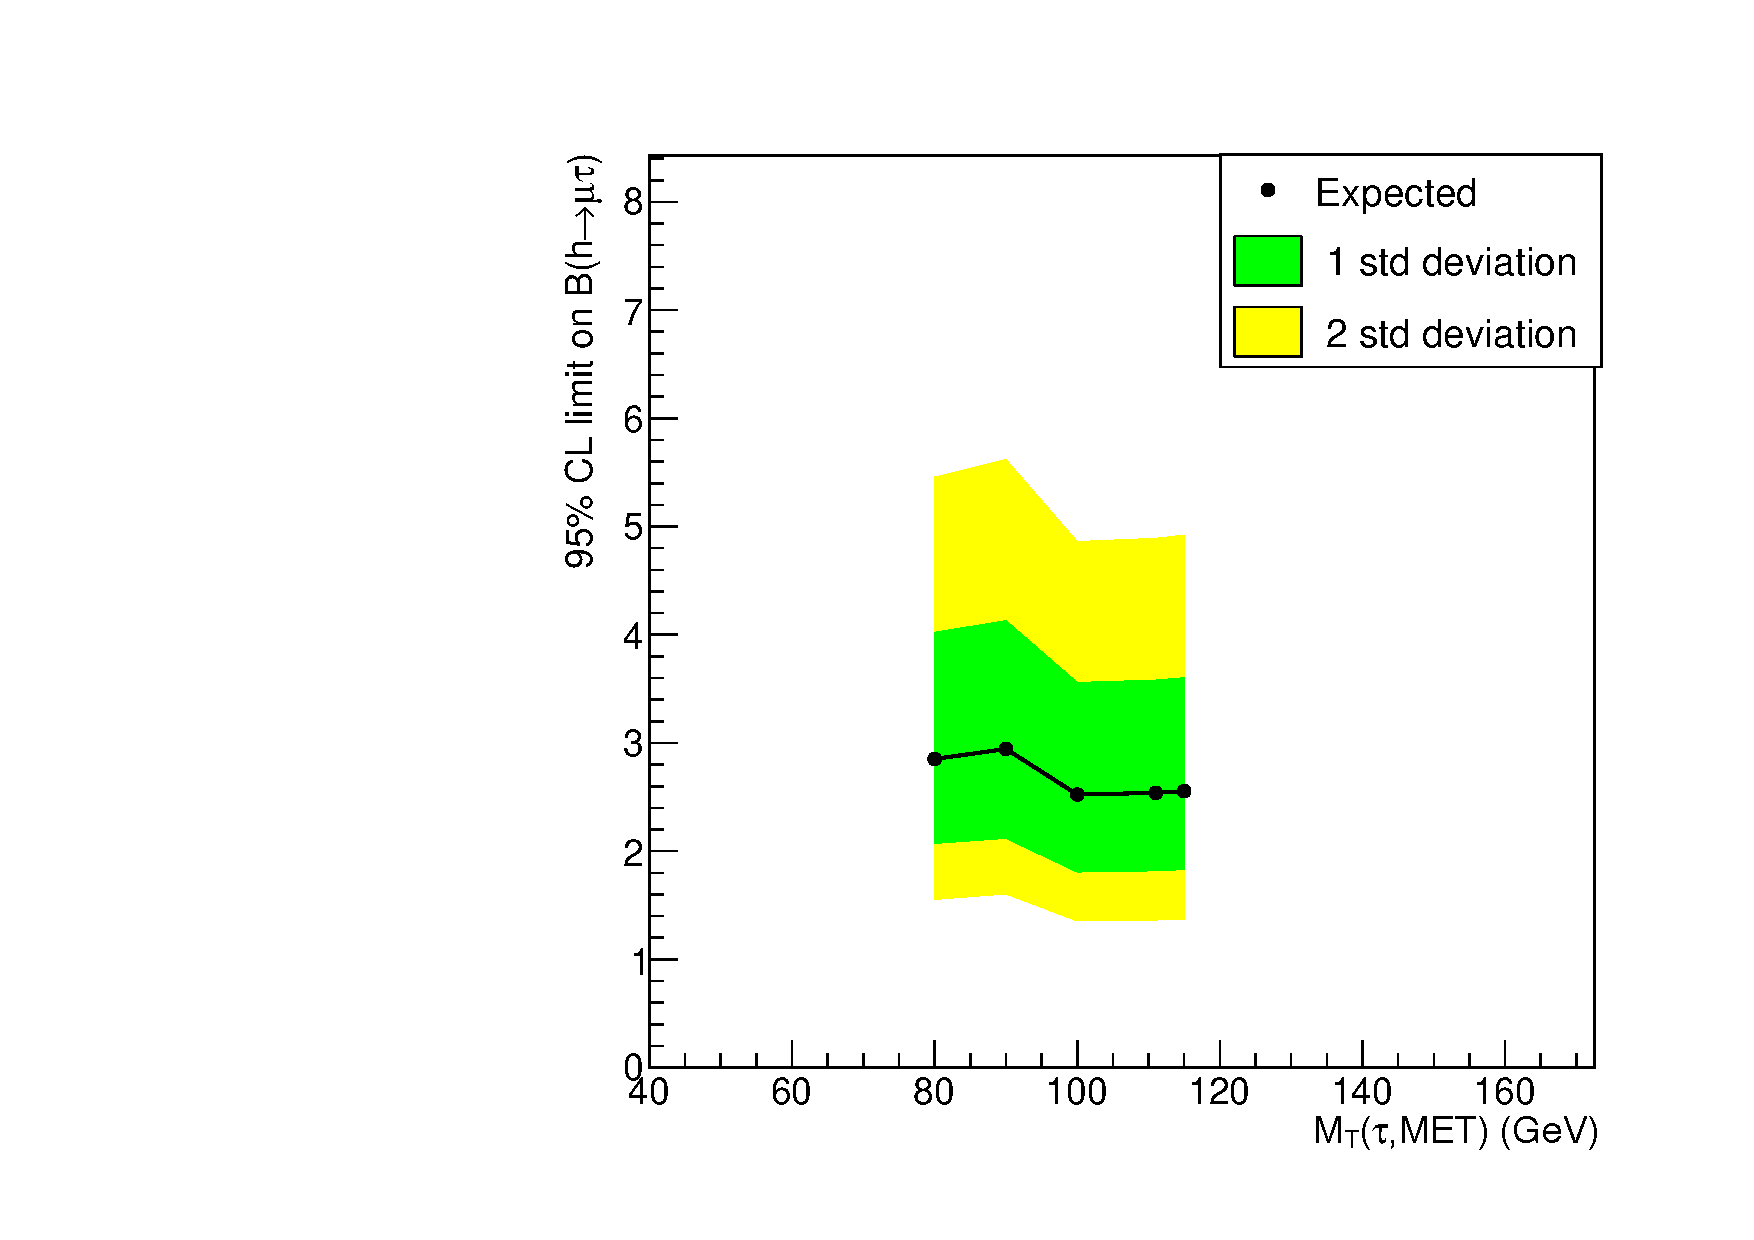
\includegraphics[width=0.4\textwidth]{chapter5/Tuning/vbf_ggtMtToPfMet_type1.pdf}}
     \subfigure[2 jets, VBF-enriched]{ 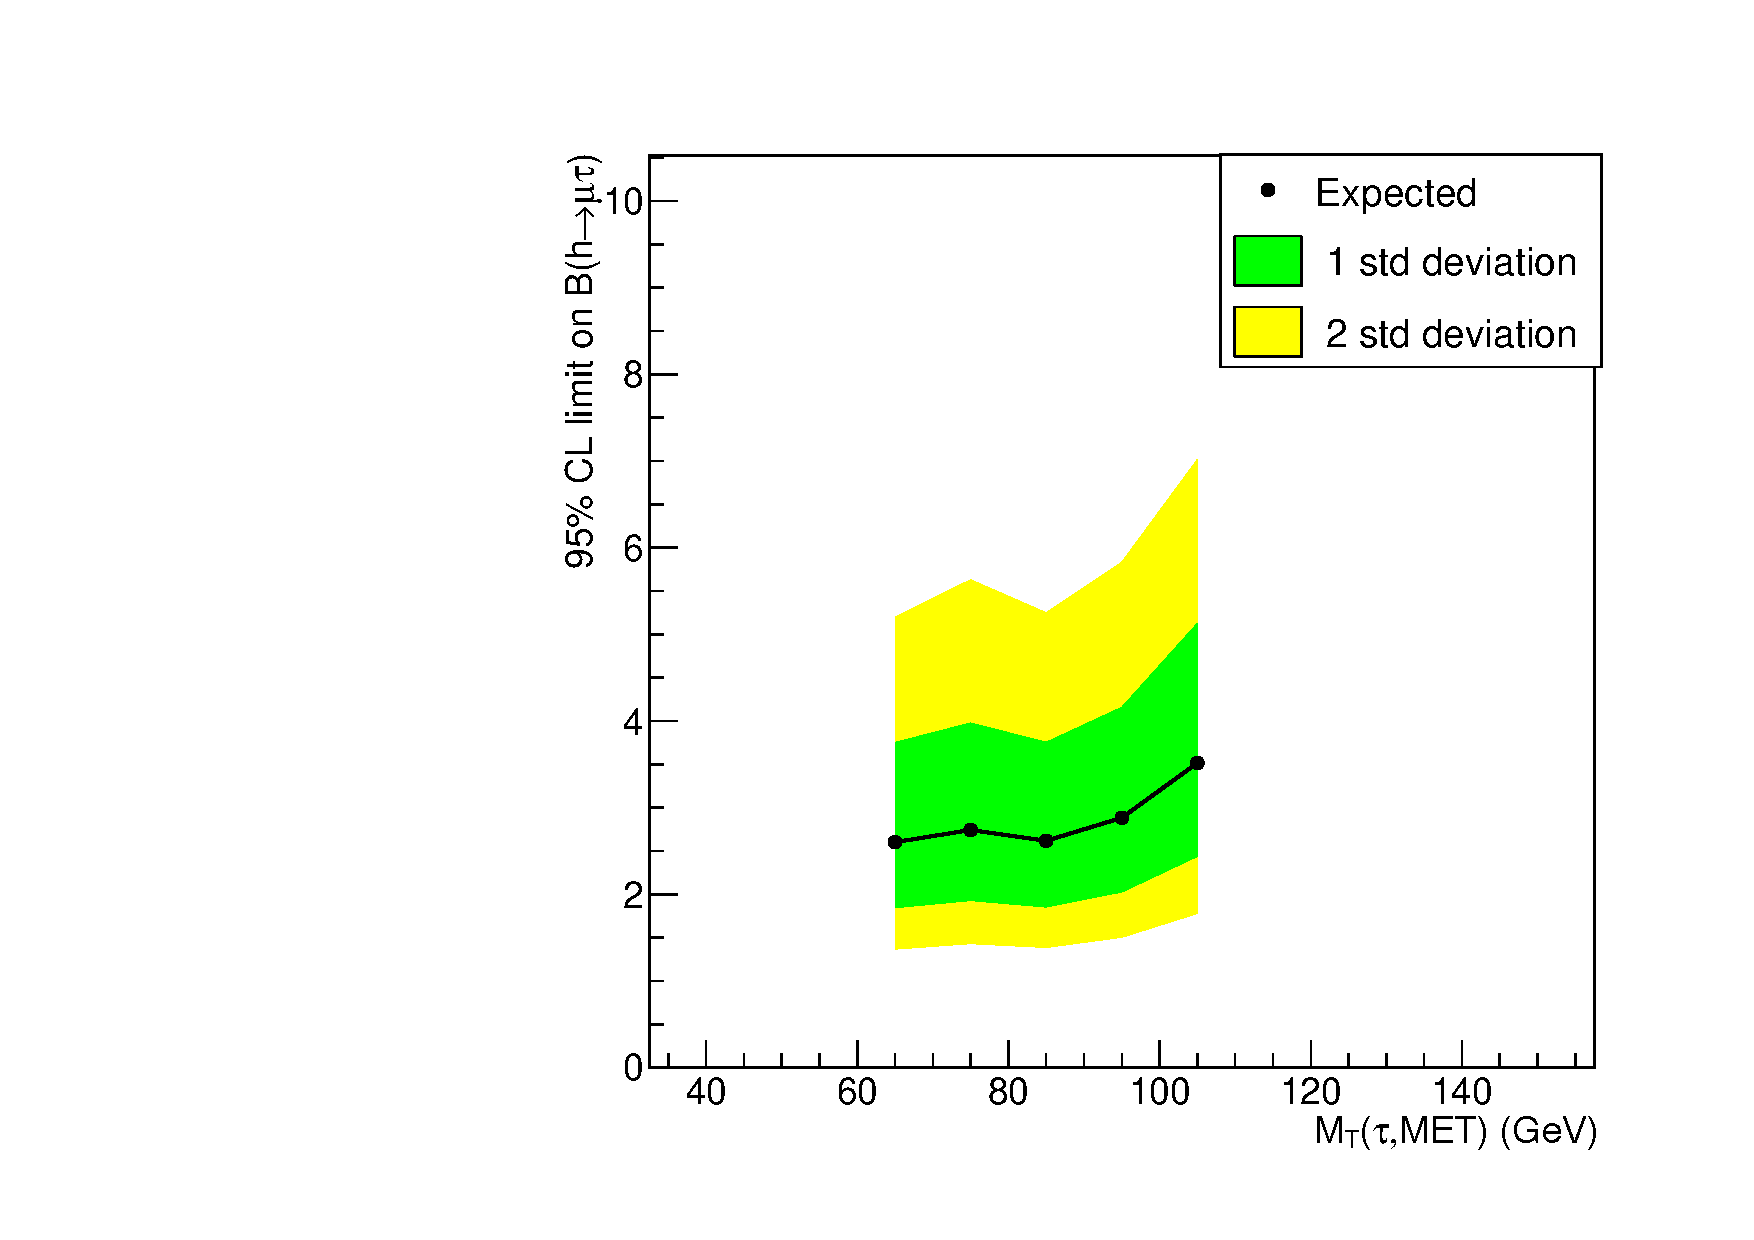
\includegraphics[width=0.4\textwidth]{chapter5/Tuning/vbf_vbftMtToPfMet_type1.pdf}}
     \caption{Expected limits based on an Asimov dataset as a function of $M_T(\tau, MET)$ for the different categories.}
     \label{fig:optMT}
\end{figure}

\begin{figure}[!tbp] 
\centering
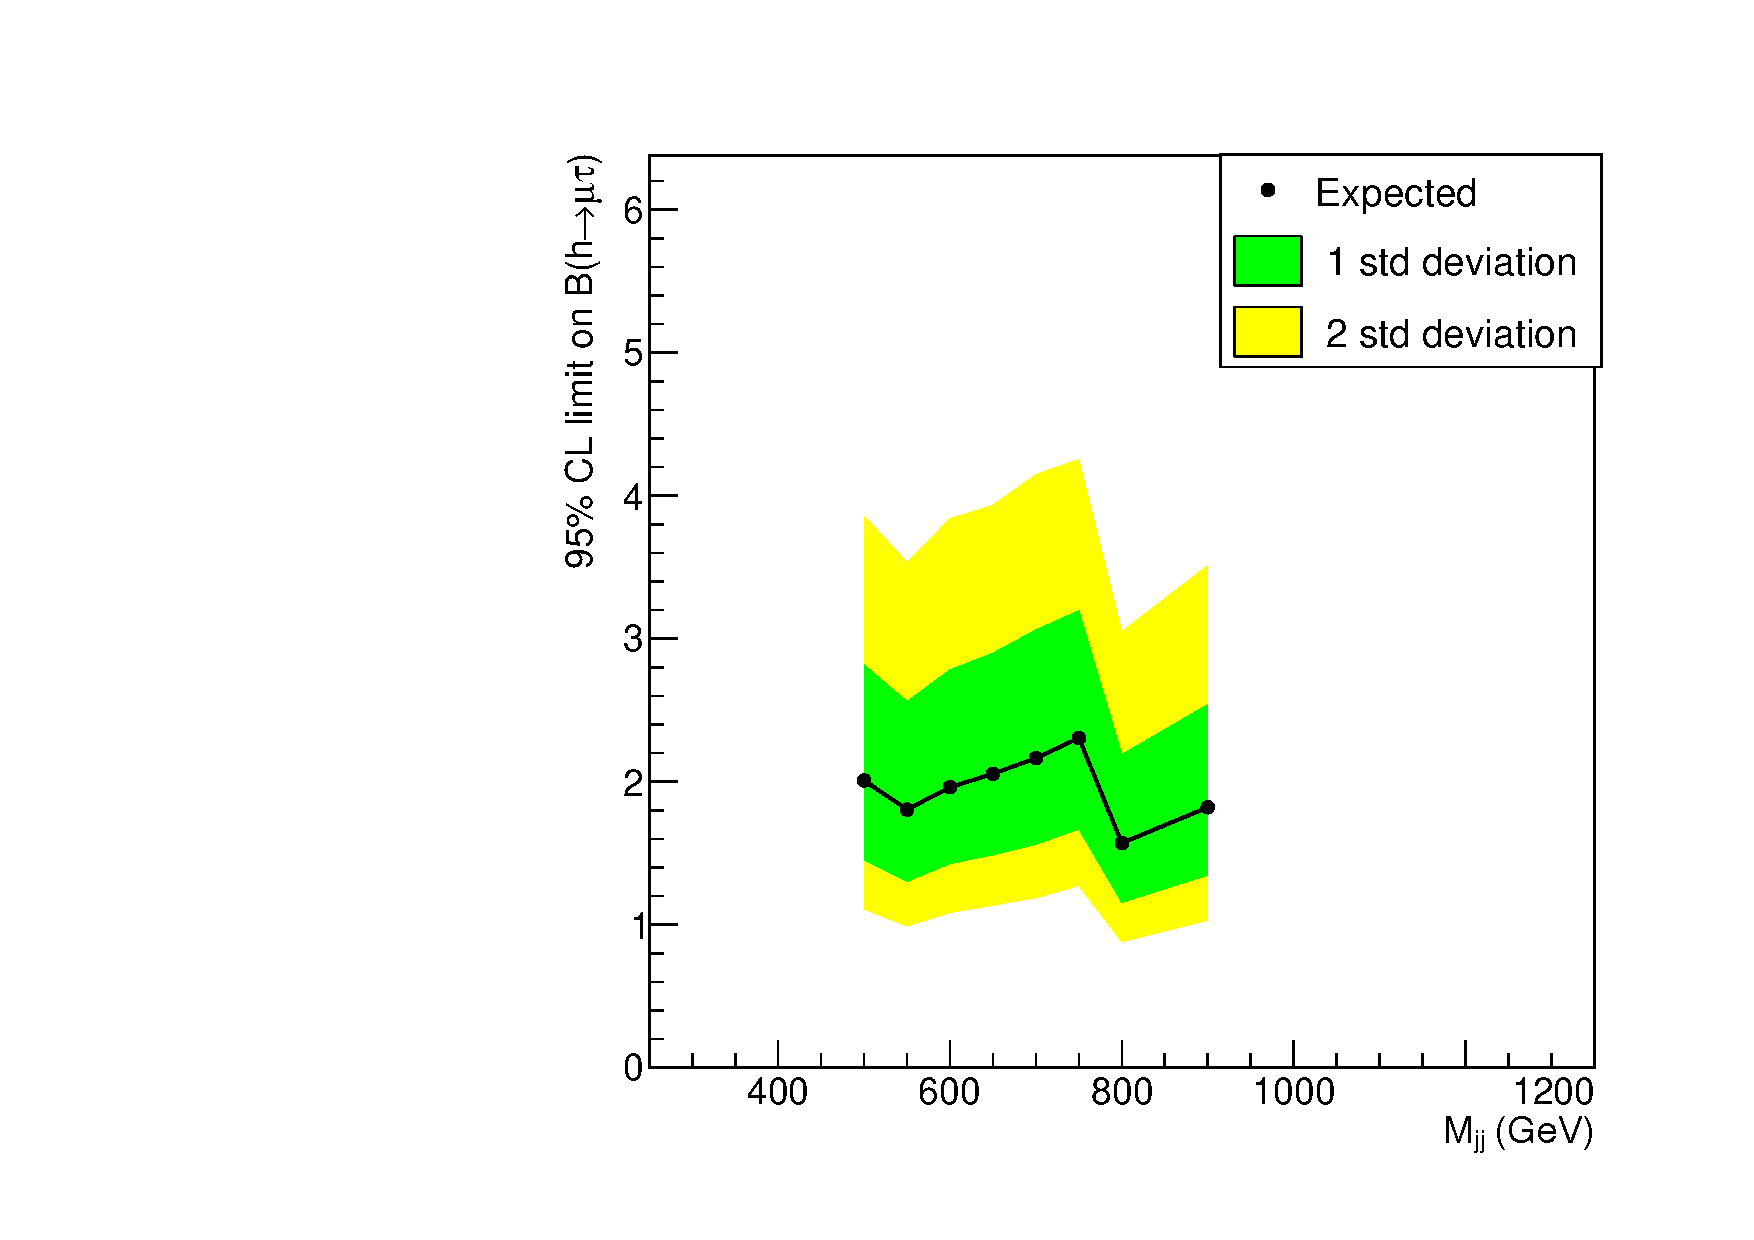
\includegraphics[width=0.4\textwidth]{chapter5/Tuning/vbf_vbfvbfMass.pdf}
\caption{Expected limits based on an Asimov dataset as a function of $M_{jj}$ for the 2 jet categories.}
\label{fig:optVBFmass}
\end{figure}



\begin{table}[hbtp]
  \begin{center}
  \caption{Selection criteria in each category with the optimization of the $\Hmuhad$ analysis}
  \begin{tabular}{l} \hline
  {\bf 0-jet category} \\ \hline
  \tabitem $\pt^{\mu}>26$ GeV, $\pt^{\tau}>30$ GeV\\
  \tabitem $M_T(\tau)<105$ GeV \\
  \tabitem No jets with $\pt^{jet}>30$ GeV, $|\eta|<4.7$, LooseID \\ \hline
 {\bf 1-jet category} \\ \hline
  \tabitem $\pt^{\mu}>26$ GeV, $\pt^{\tau}>30$ GeV \\
  \tabitem $M_T(\tau)<105$ GeV \\
  \tabitem One jet  with $\pt^{jet}>30$ GeV, $|\eta|<4.7$, LooseID
  \\ \hline
  {\bf 2-jet, gg-enriched category} \\ \hline
  \tabitem $\pt^{\mu}>26$ GeV, $\pt^{\tau}>30$ GeV \\
  \tabitem $M_T(\tau)<105$ GeV \\
      \tabitem $\pt^{jet1}>30$ GeV,$\pt^{jet2}>30$ GeV
      $|\eta_{jet1}|<4.7$,$|\eta_{jet2}|<4.7$, LooseID\\
      \tabitem $M_{jj}<550$ GeV\\
      \tabitem Two jets with $\pt^{jet}>30$ GeV, $|\eta|<4.7$, LooseID\\ \hline
  {\bf 2-jet, VBF-enriched category} \\ \hline
  \tabitem $\pt^{\mu}>26$ GeV, $\pt^{\tau}>30$ GeV \\
  \tabitem $M_T(\tau)<85$ GeV \\
      \tabitem $\pt^{jet1}>30$ GeV,$\pt^{jet2}>30$ GeV
      $|\eta_{jet1}|<4.7$,$|\eta_{jet2}|<4.7$, LooseID\\
      \tabitem $M_{jj}>550$ GeV\\
      \tabitem Two jets with $\pt^{jet}>30$ GeV, $|\eta|<4.7$, LooseID\\ \hline
  \label{tab:Mhadcategories}
\end{tabular}
\end{center}
\end{table}




\subsection{Multivariate analysis}
A boosted decision trees(BDT) method is used as the multivariate analysis method in the $H\rightarrow\mu\tau_h$ search which is more sensitive than the $\mcol$ fit analysis. The BDT algorithm used in this search is implemented in the TMVA package \cite{TMVAnote}. BDT takes in signal and background datasets with a selected set of input variables. Input variables are the ones that show distinguishing power between signal and backgrounds. The training output is a weight file, which contains a list of weights to indicate how likely an event is signal-like with a give set of input variables. A more detail description of the BDT method is available in section \ref{BDTchaper}.  In this analysis, signal and background events are required to pass the loose selection criteria. All of the categories are combined. The signal events from the ggH and VBF Higgs production mode are mixed by weighting with respect to their production cross section. The background sample used in the training is the misidentified lepton background from the like sign region(Region II as in Table.~\ref{tab:fakeratediagram}). The list of BDT input variables  is in the following list and the distribution of the variables are shown in Fig.~\ref{fig:BDT_input_var_mutauhad}.

\begin{itemize}
\item Transverse mass between the $\tauh$ and $\ETmiss$, $M_{T}(\tau_{h})$.
\item Missing transverse energy, $\ETmiss$.
\item Pseudorapidity difference between the $\mu$ and the $\tauh$ candidate, $\Delta\eta(\mu, \tauh)$.
\item Azimutal angle between the $\mu$ and the $\tauh$, $\Delta\phi (\mu,\tauh)$.
\item Azimutal angle between the $\tauh$ and the $\ETmiss$, $\Delta\phi(\tau_h,\ETmiss)$.
\item Collinear mass, $\mcol$.
\item Muon $\pt$.
\item $\tau_h$ $\pt$.
\end{itemize}

\begin{figure}[htpb]\centering
 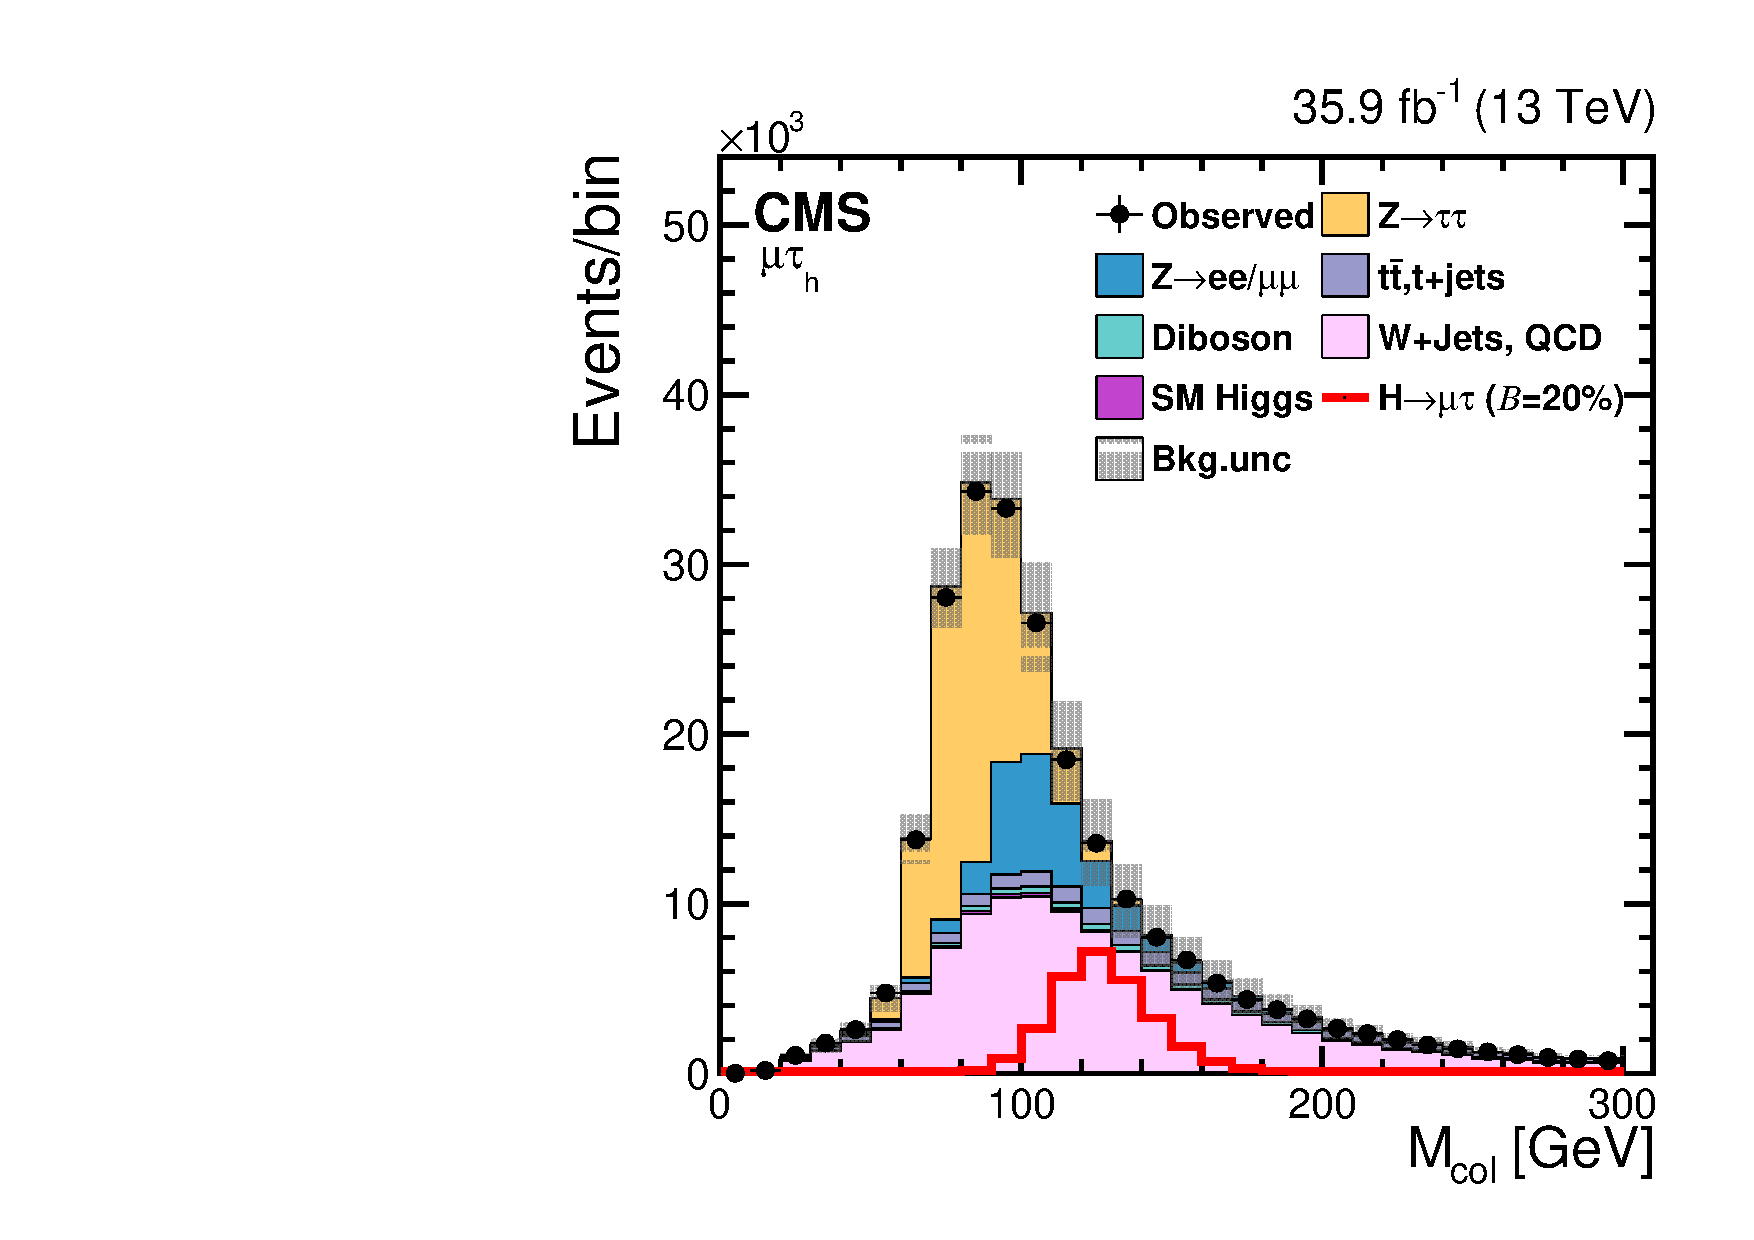
\includegraphics[width=0.315\textwidth]{chapter5/BDTvariable/LFV_preselection_collMass_type1_Fakes_PoissonErrors.pdf}
 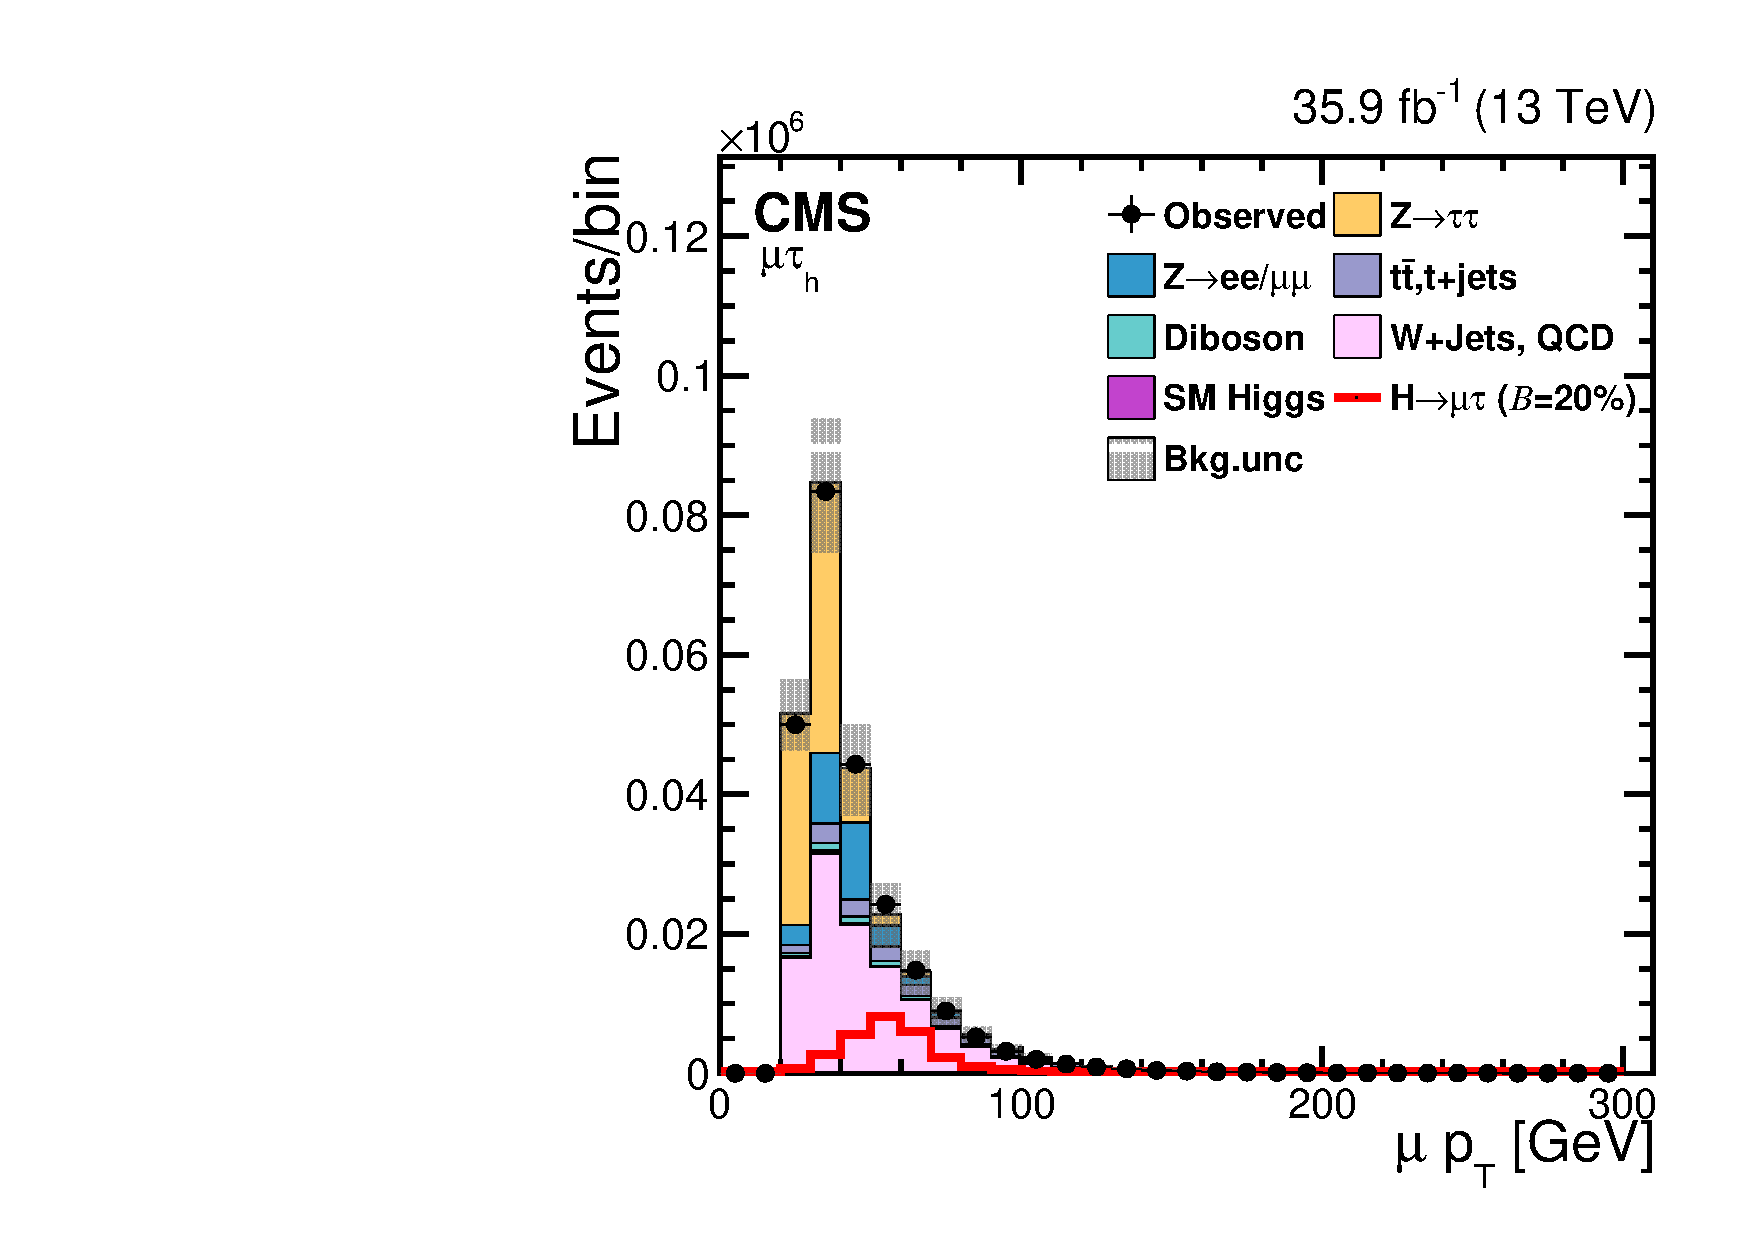
\includegraphics[width=0.315\textwidth]{chapter5/BDTvariable/LFV_preselection_mPt_Fakes_PoissonErrors.pdf} \\
 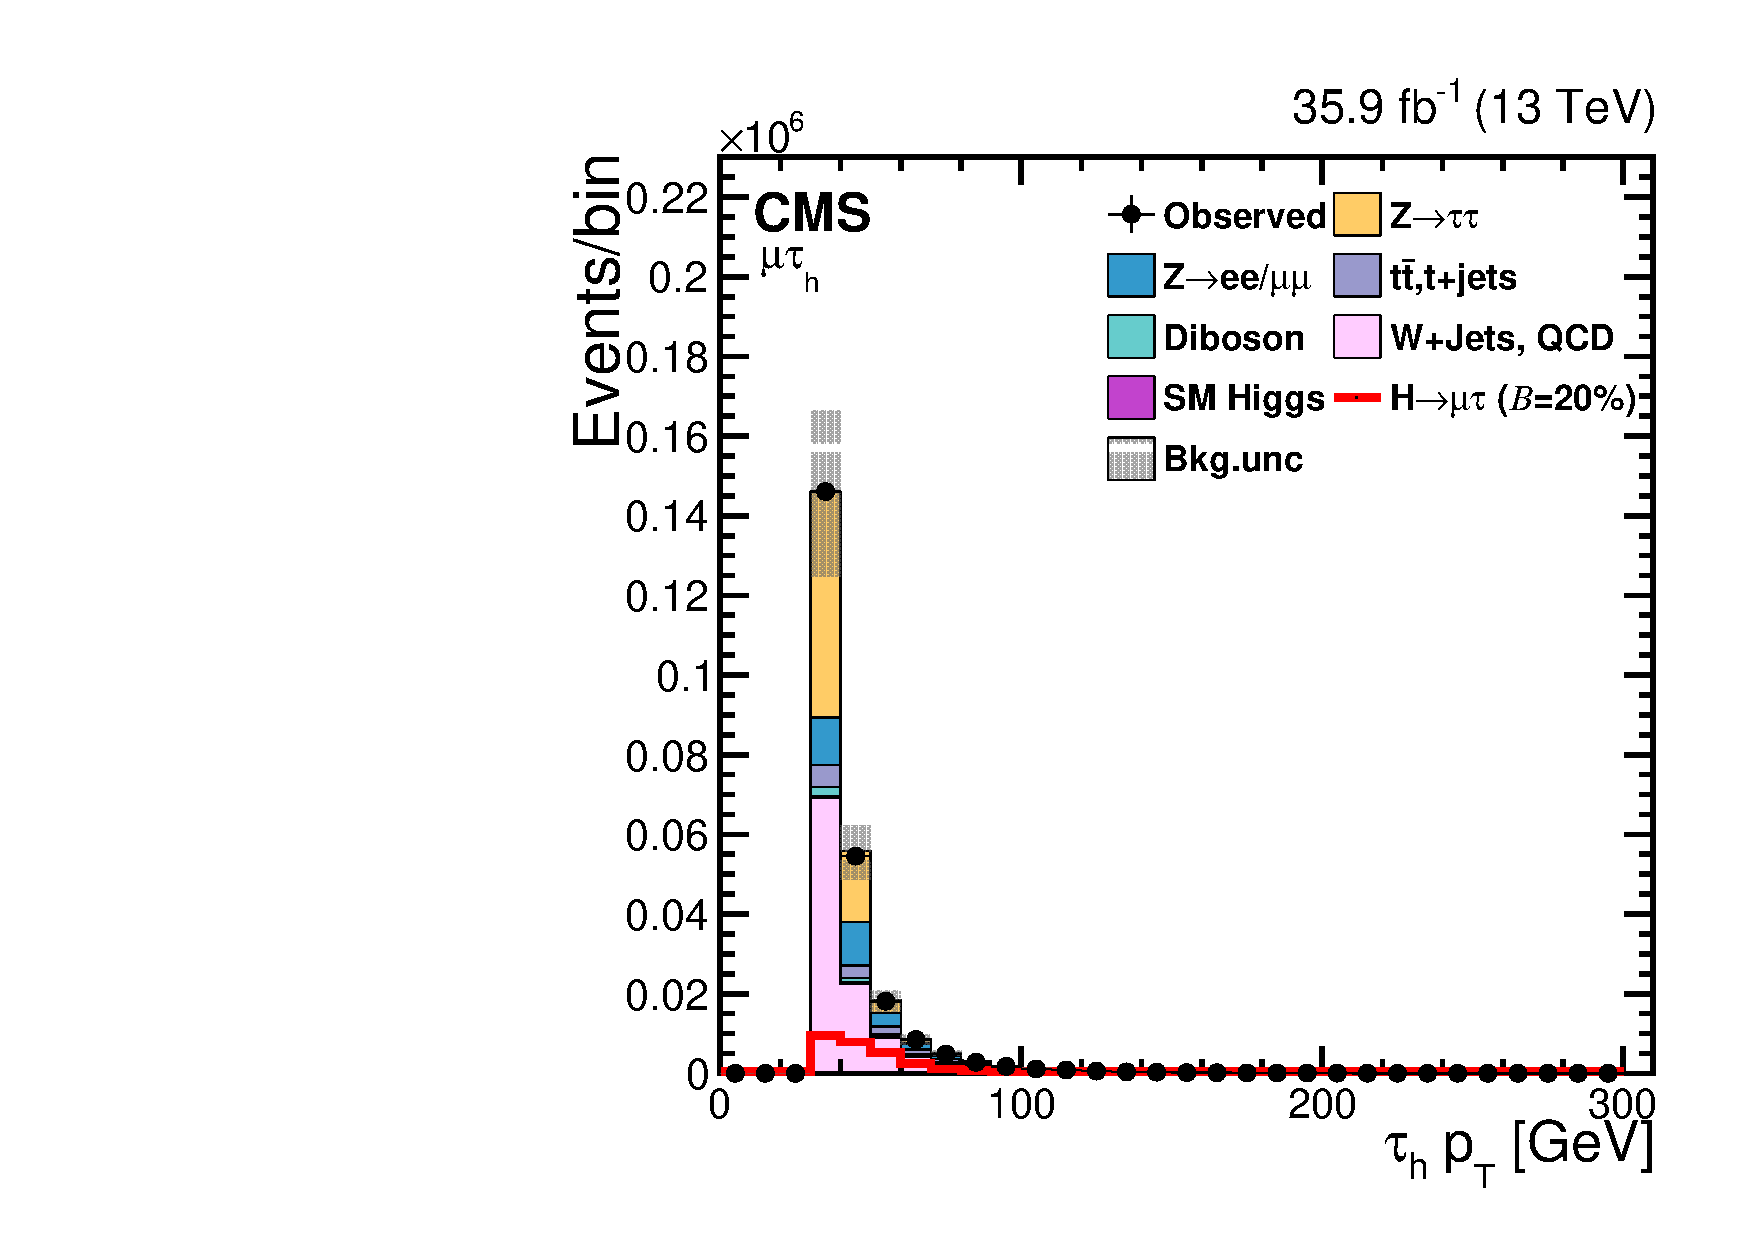
\includegraphics[width=0.315\textwidth]{chapter5/BDTvariable/LFV_preselection_tPt_Fakes_PoissonErrors.pdf}
 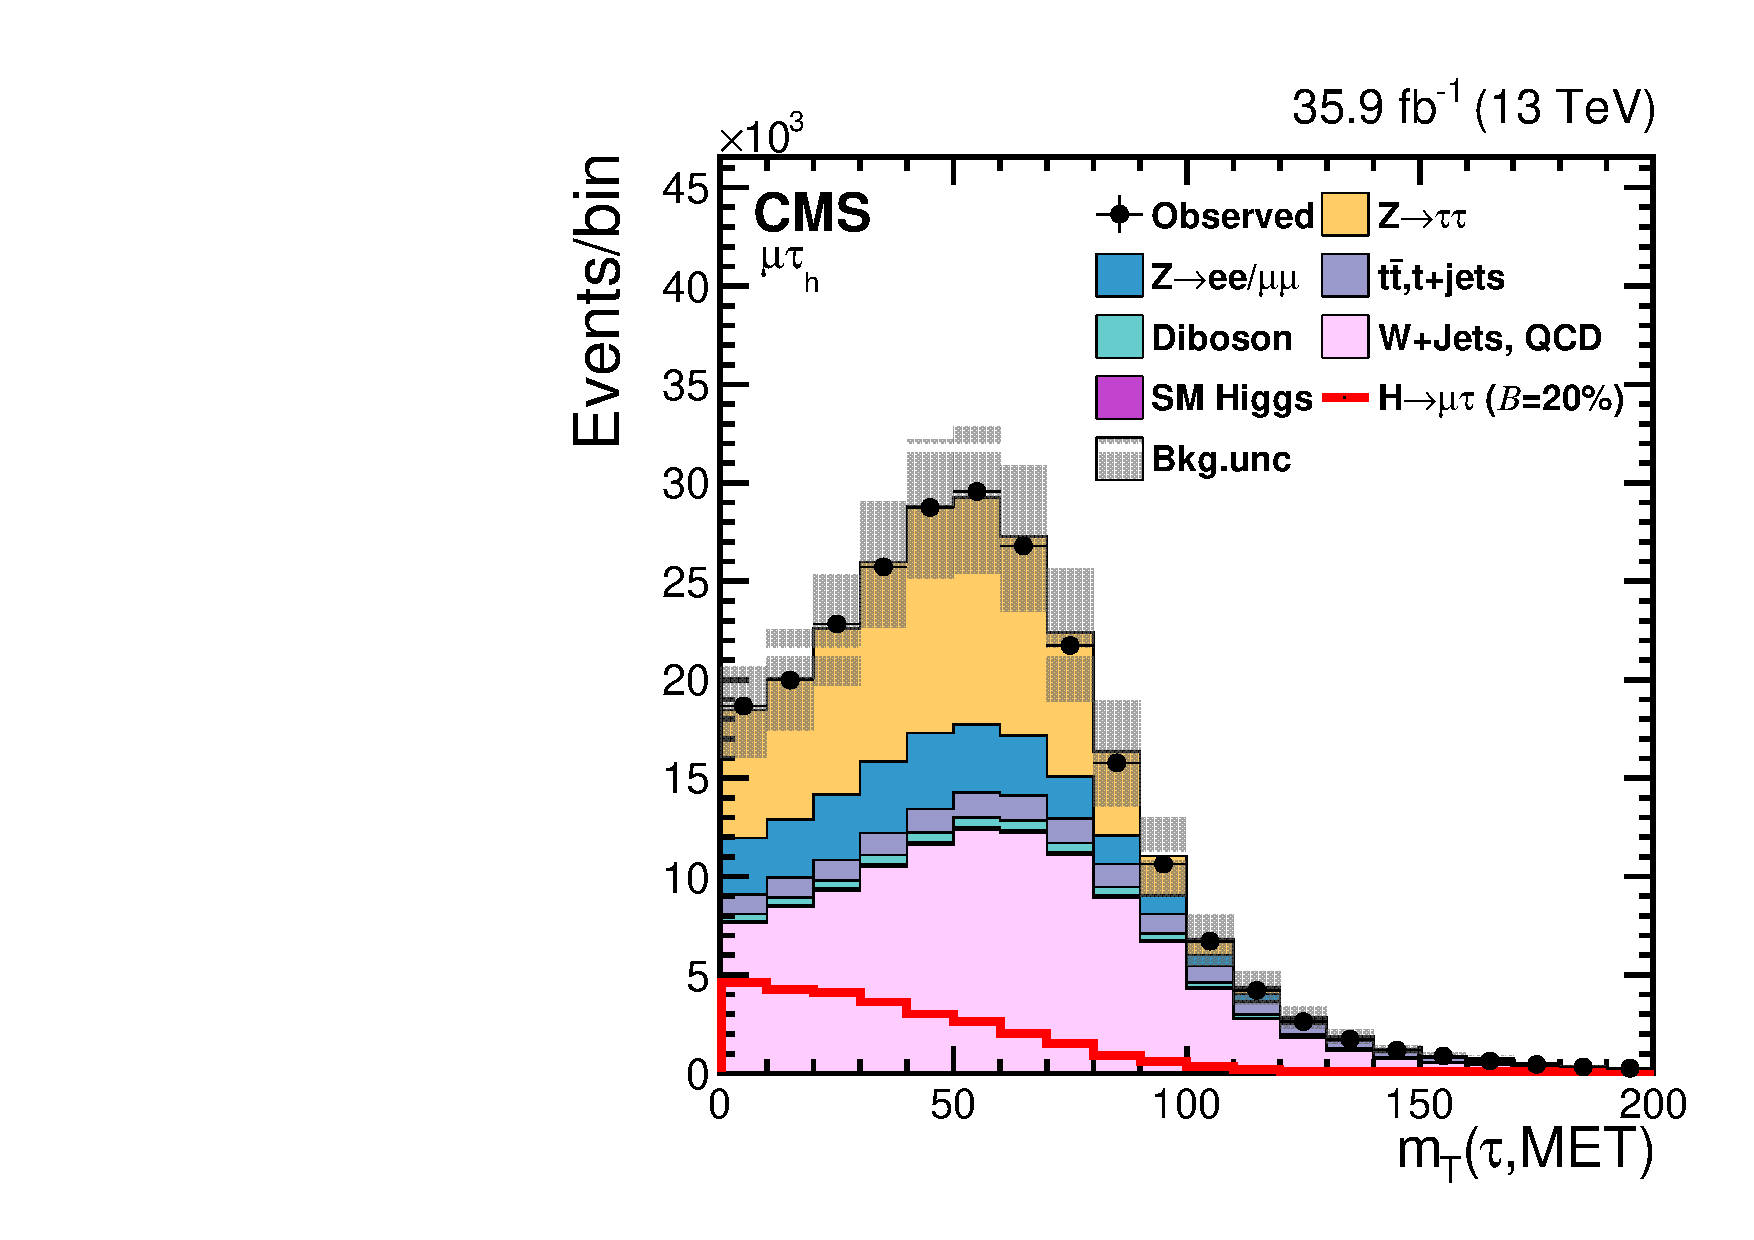
\includegraphics[width=0.315\textwidth]{chapter5/BDTvariable/LFV_preselection_tMtToPfMet_type1_Fakes_PoissonErrors.pdf}  \\
 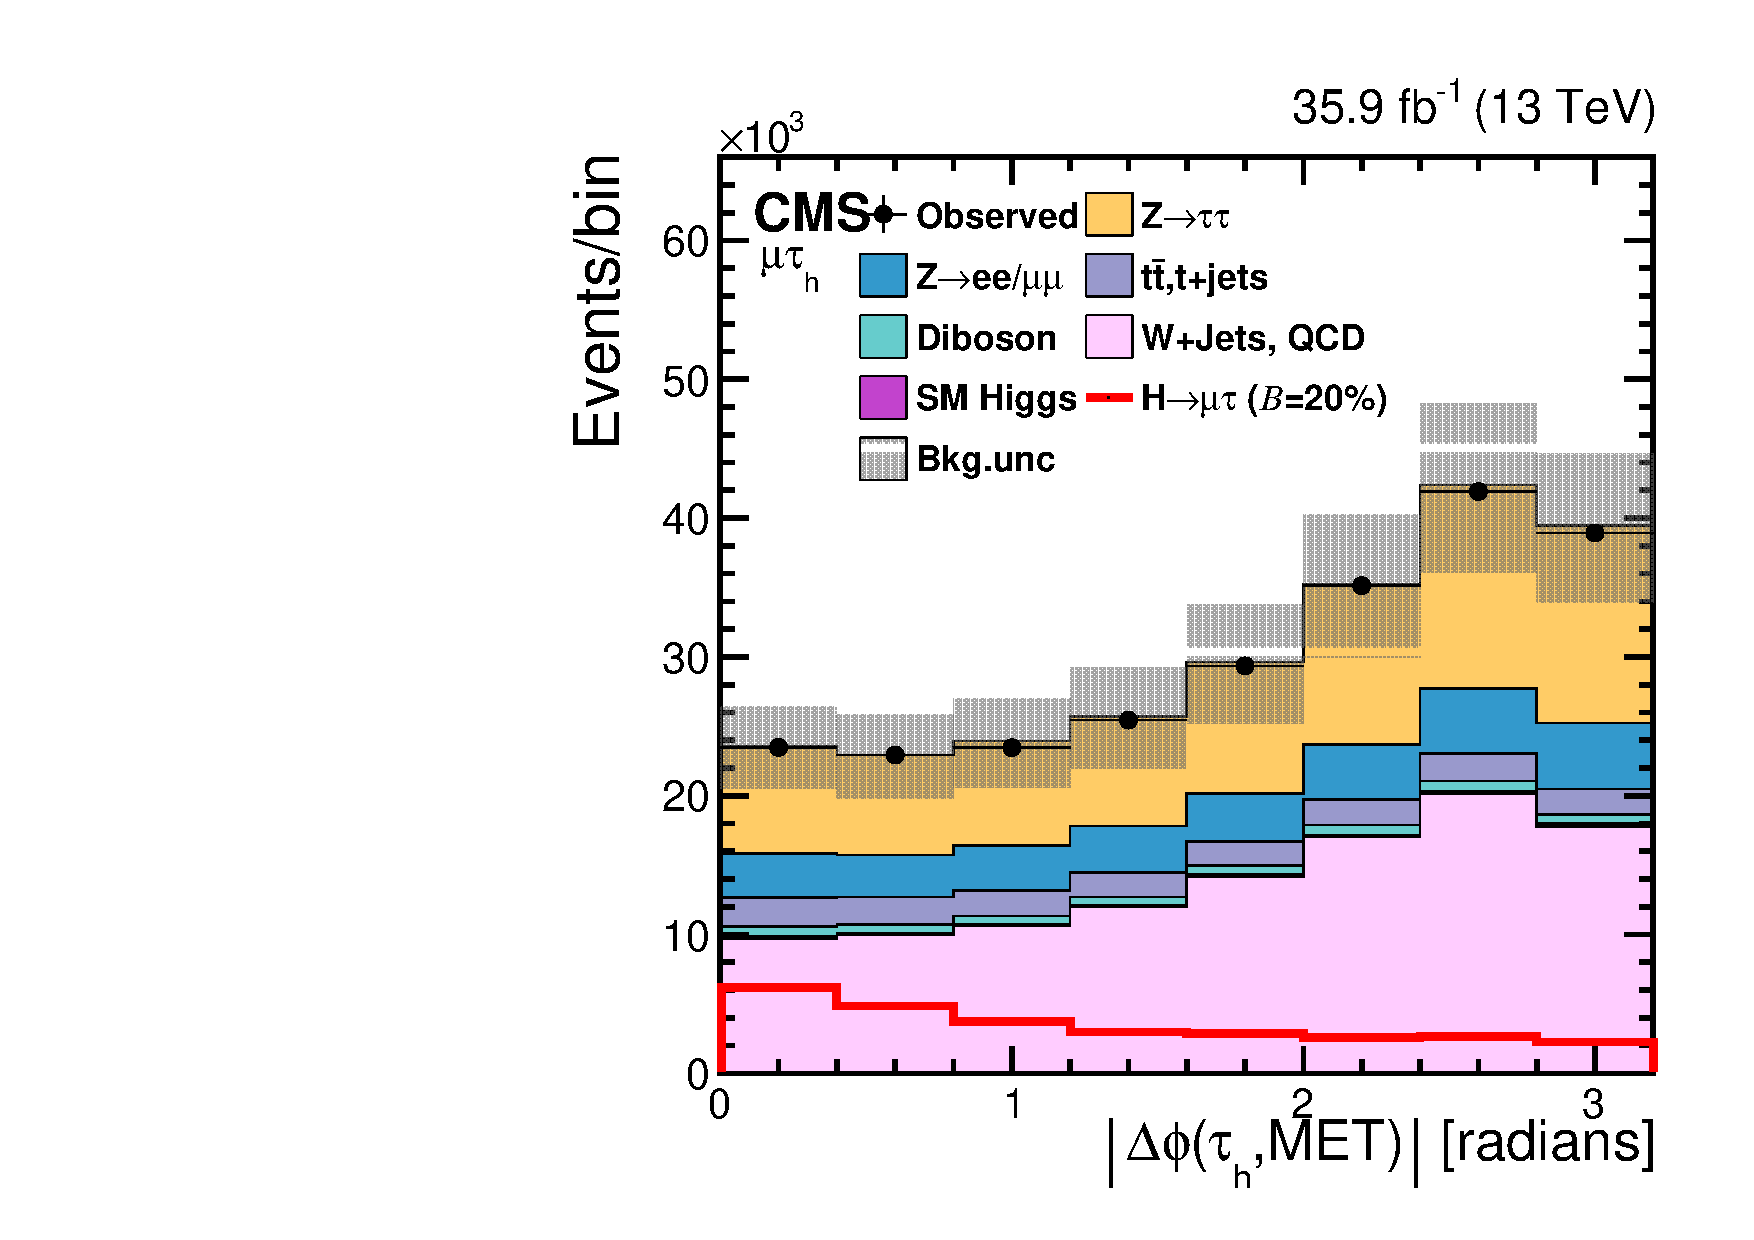
\includegraphics[width=0.315\textwidth]{chapter5/BDTvariable/LFV_preselection_tDPhiToPfMet_type1_Fakes_PoissonErrors.pdf}
 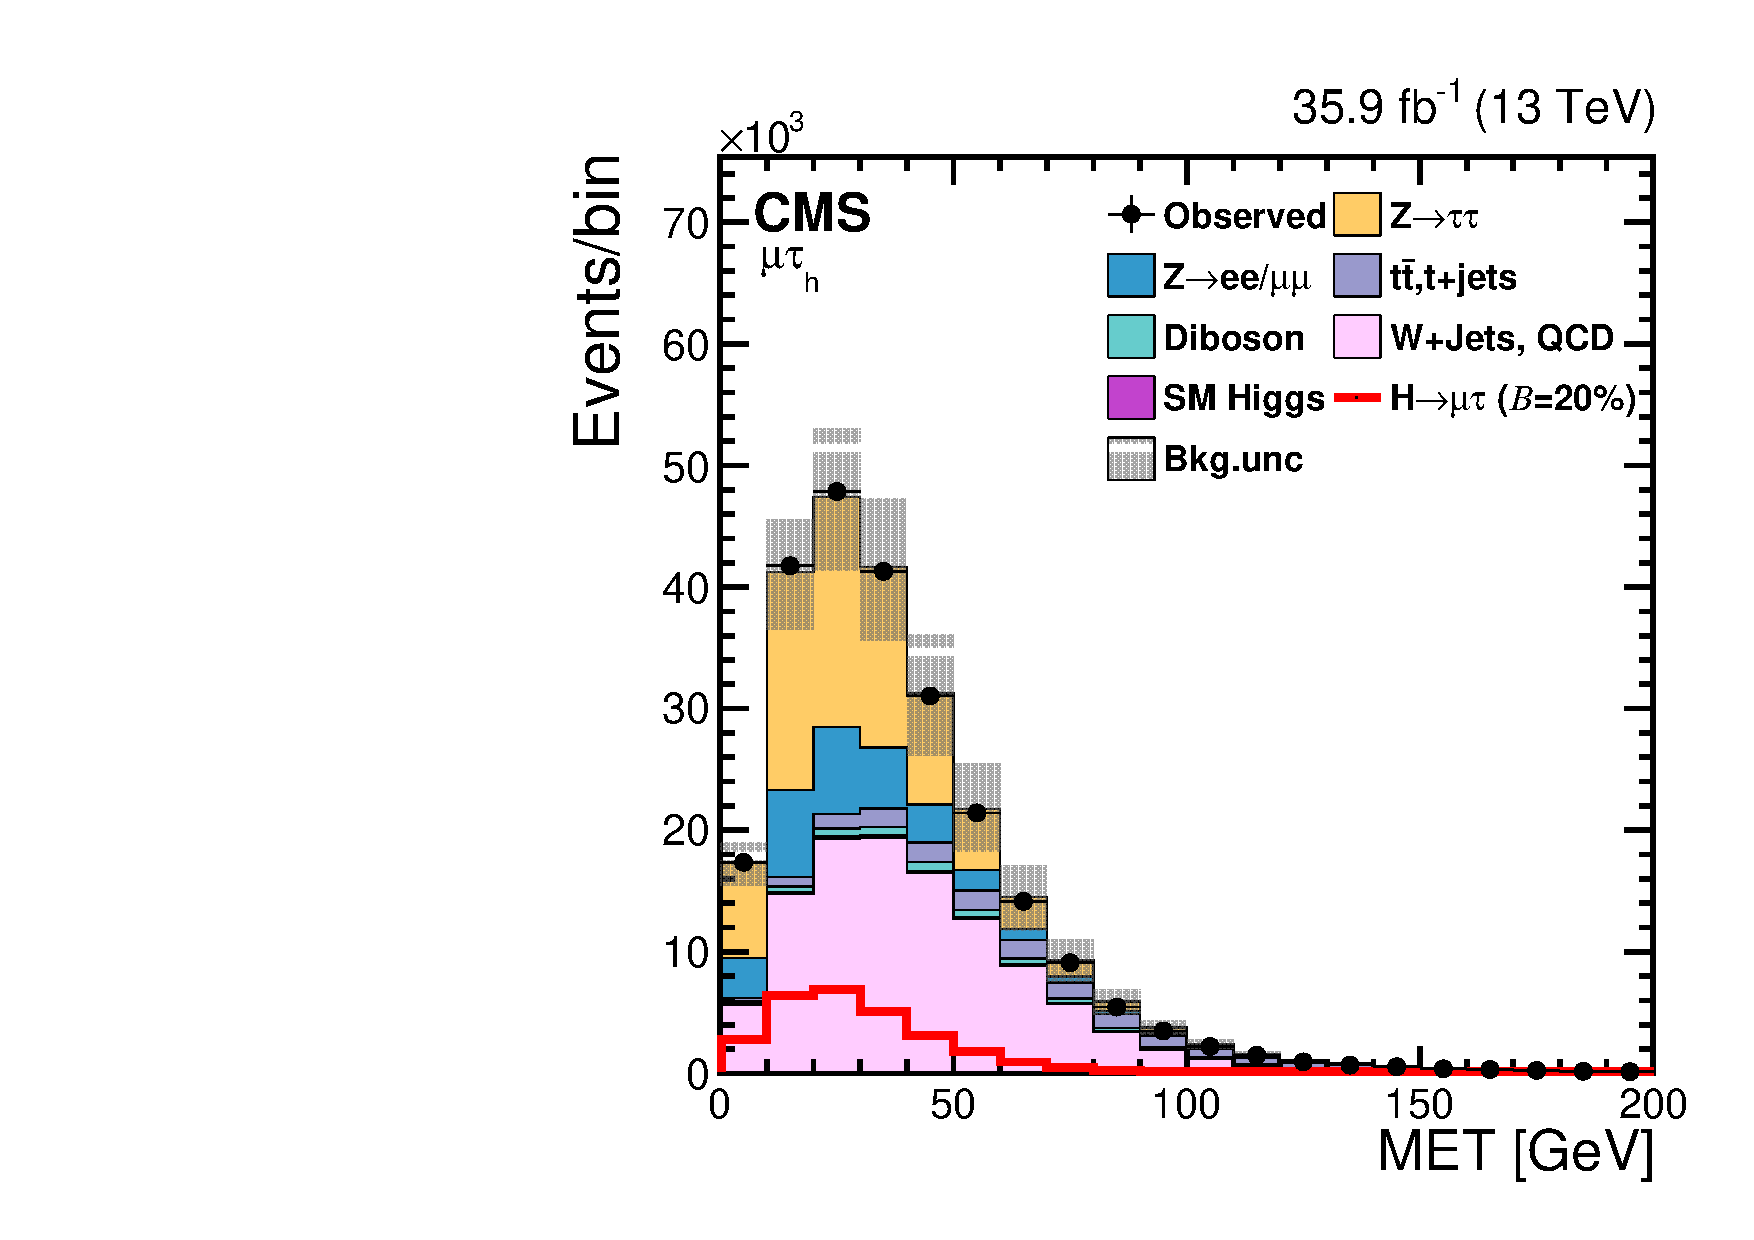
\includegraphics[width=0.315\textwidth]{chapter5/BDTvariable/LFV_preselection_type1_pfMetEt_Fakes_PoissonErrors.pdf} \\
 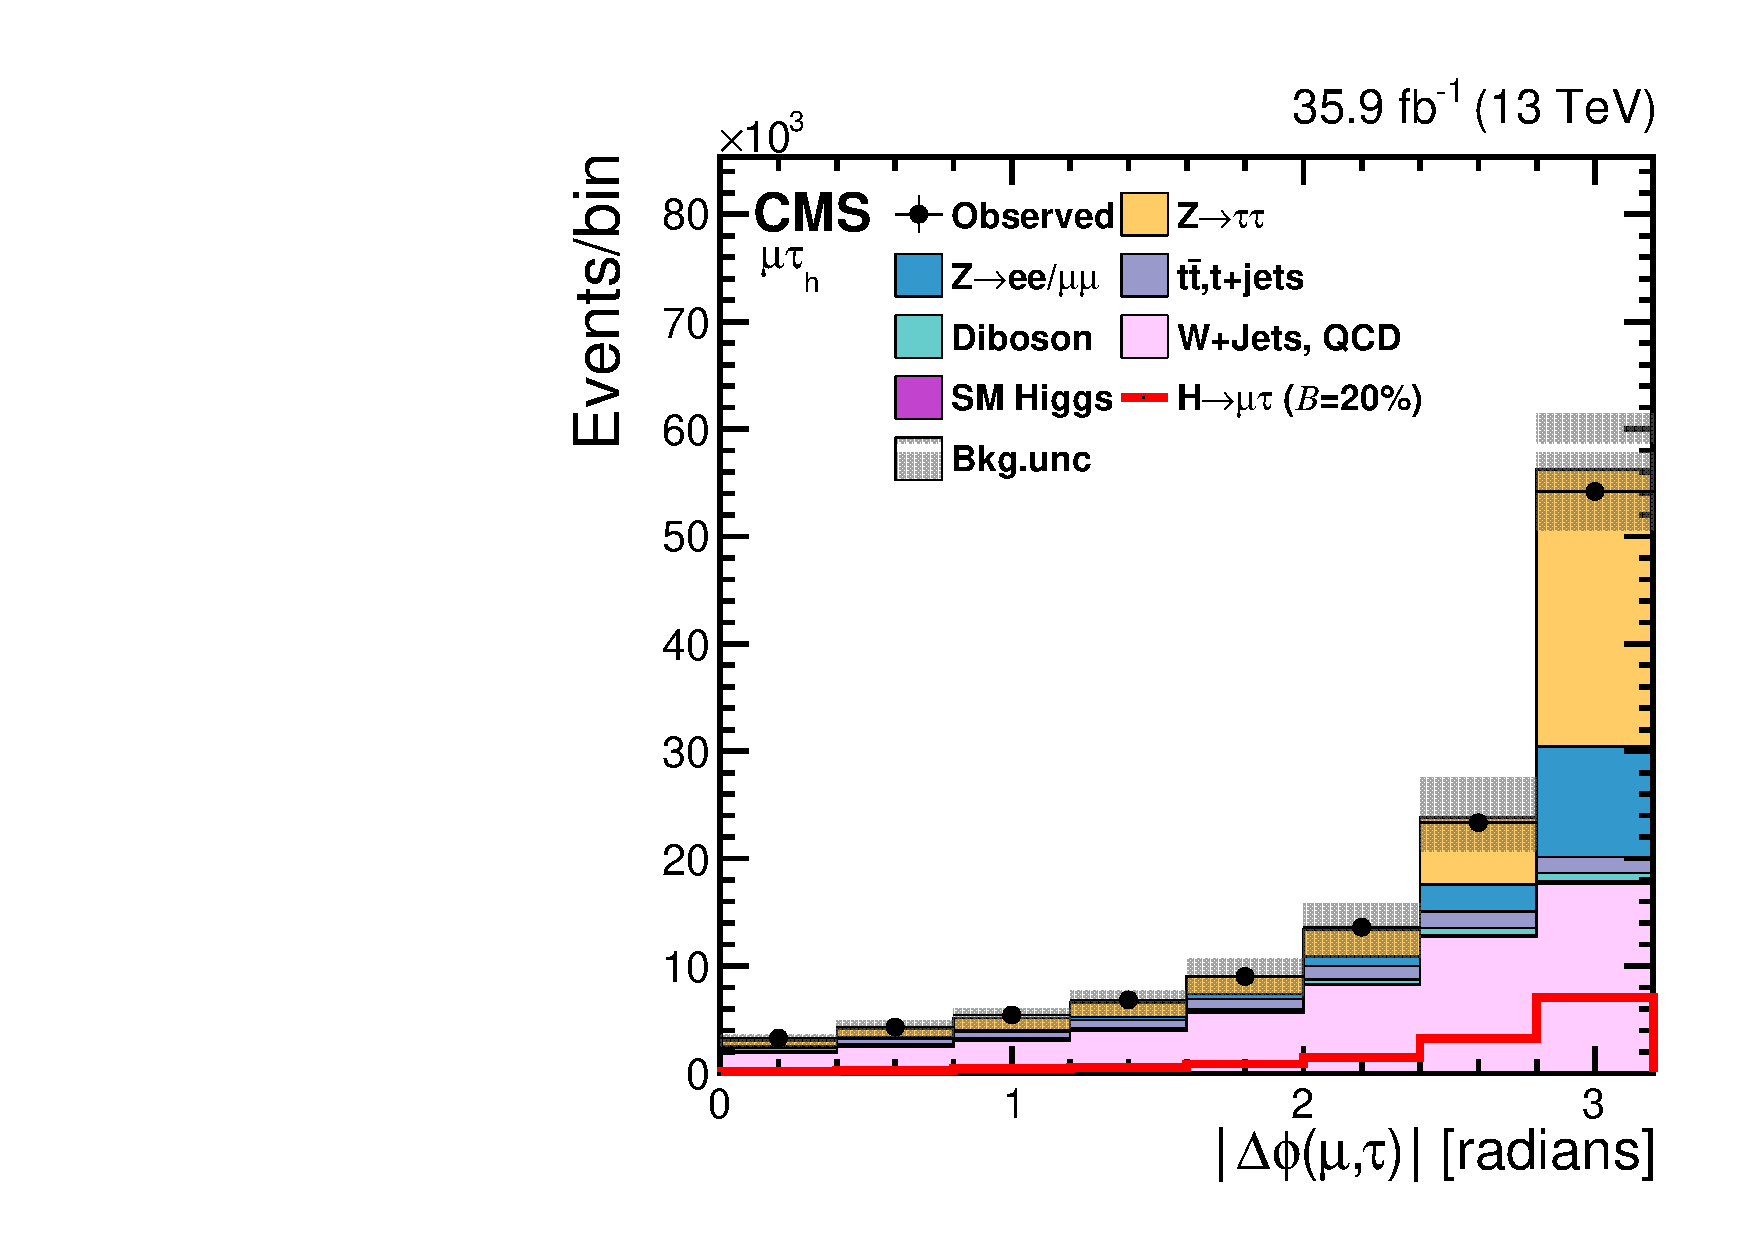
\includegraphics[width=0.315\textwidth]{chapter5/BDTvariable/LFV_preselection_m_t_DPhi_Fakes_PoissonErrors.pdf}
 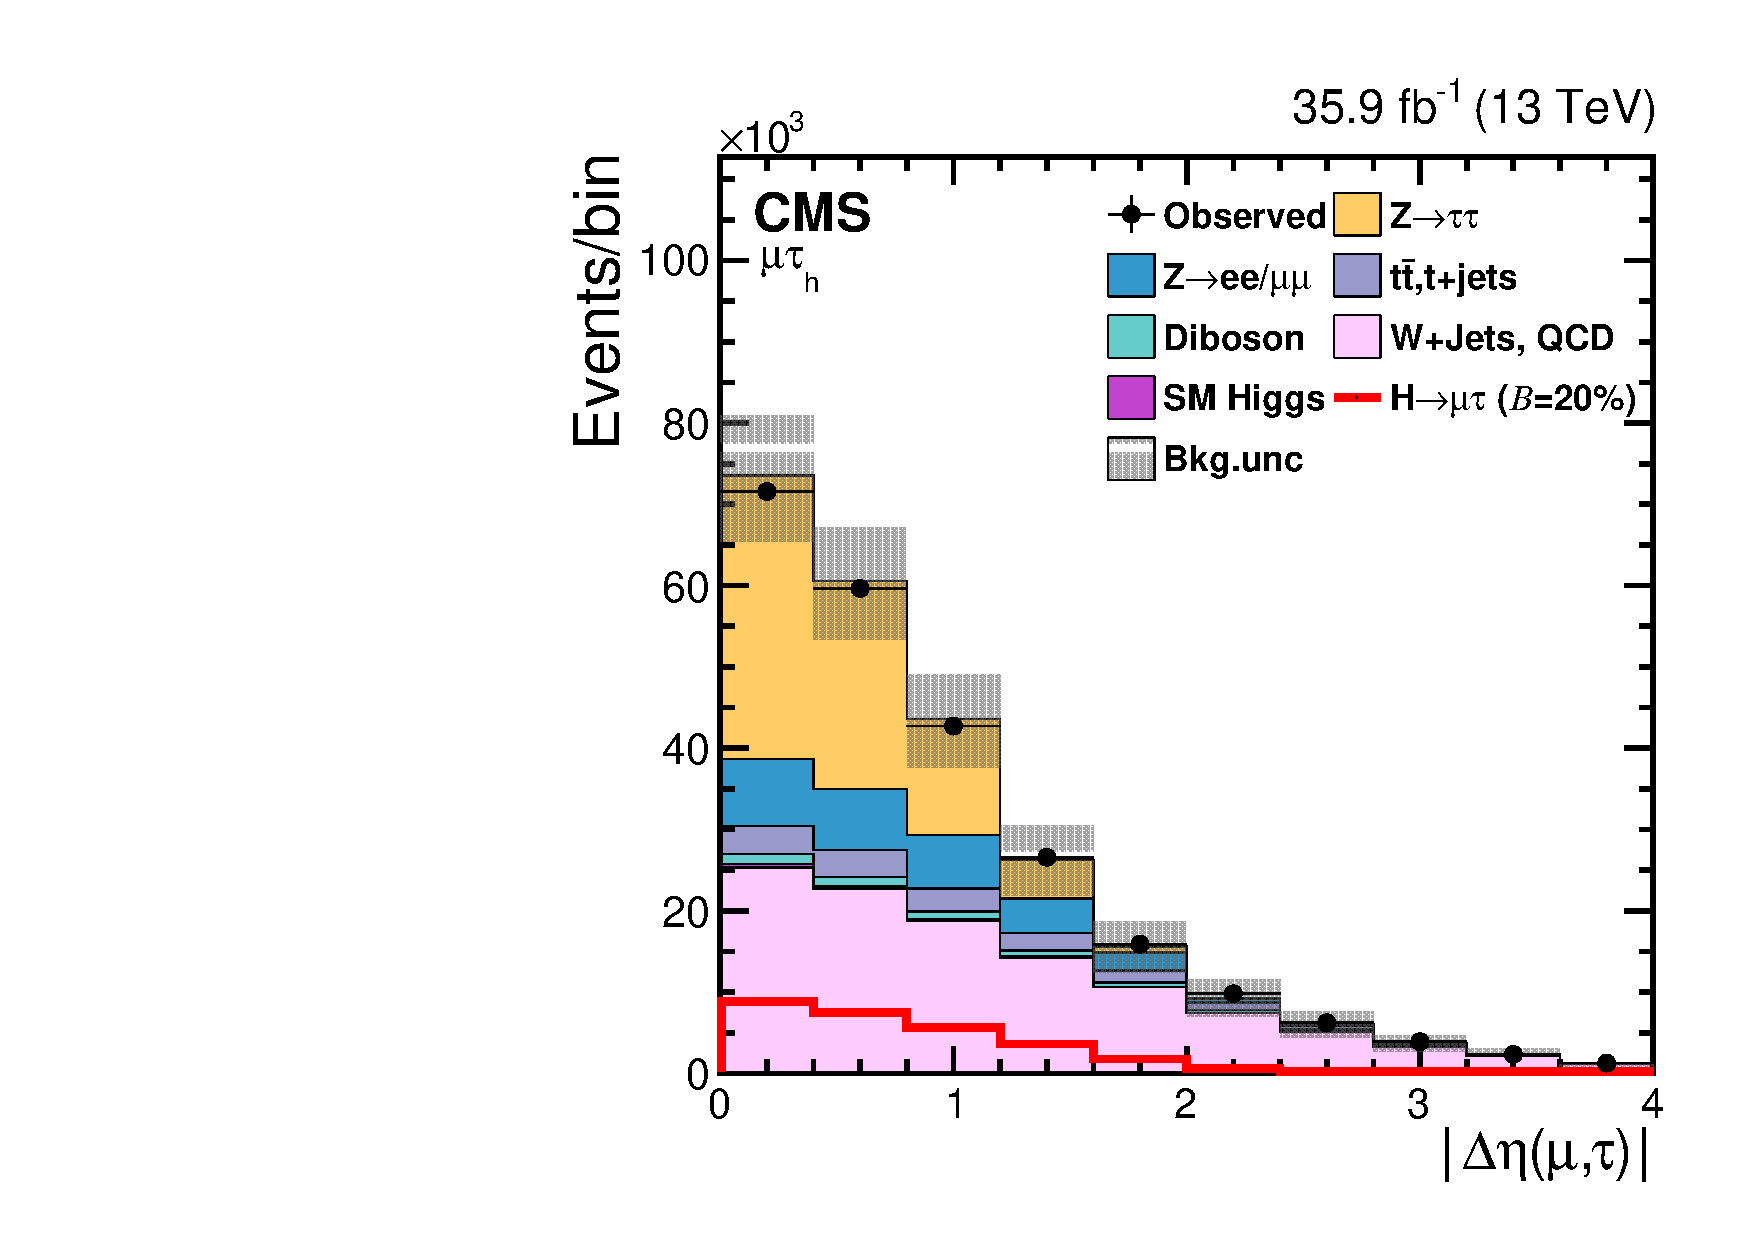
\includegraphics[width=0.315\textwidth]{chapter5/BDTvariable/LFV_preselection_m_t_DEta_Fakes_PoissonErrors.pdf}
\caption{Distributions of the  input variables to the BDT for the \Hmuhad channel.}
 \label{fig:BDT_input_var_mutauhad}
\end{figure}


\begin{figure}[htbp] 
     \centering
     \subfigure[Signal sample variables correlation]{ 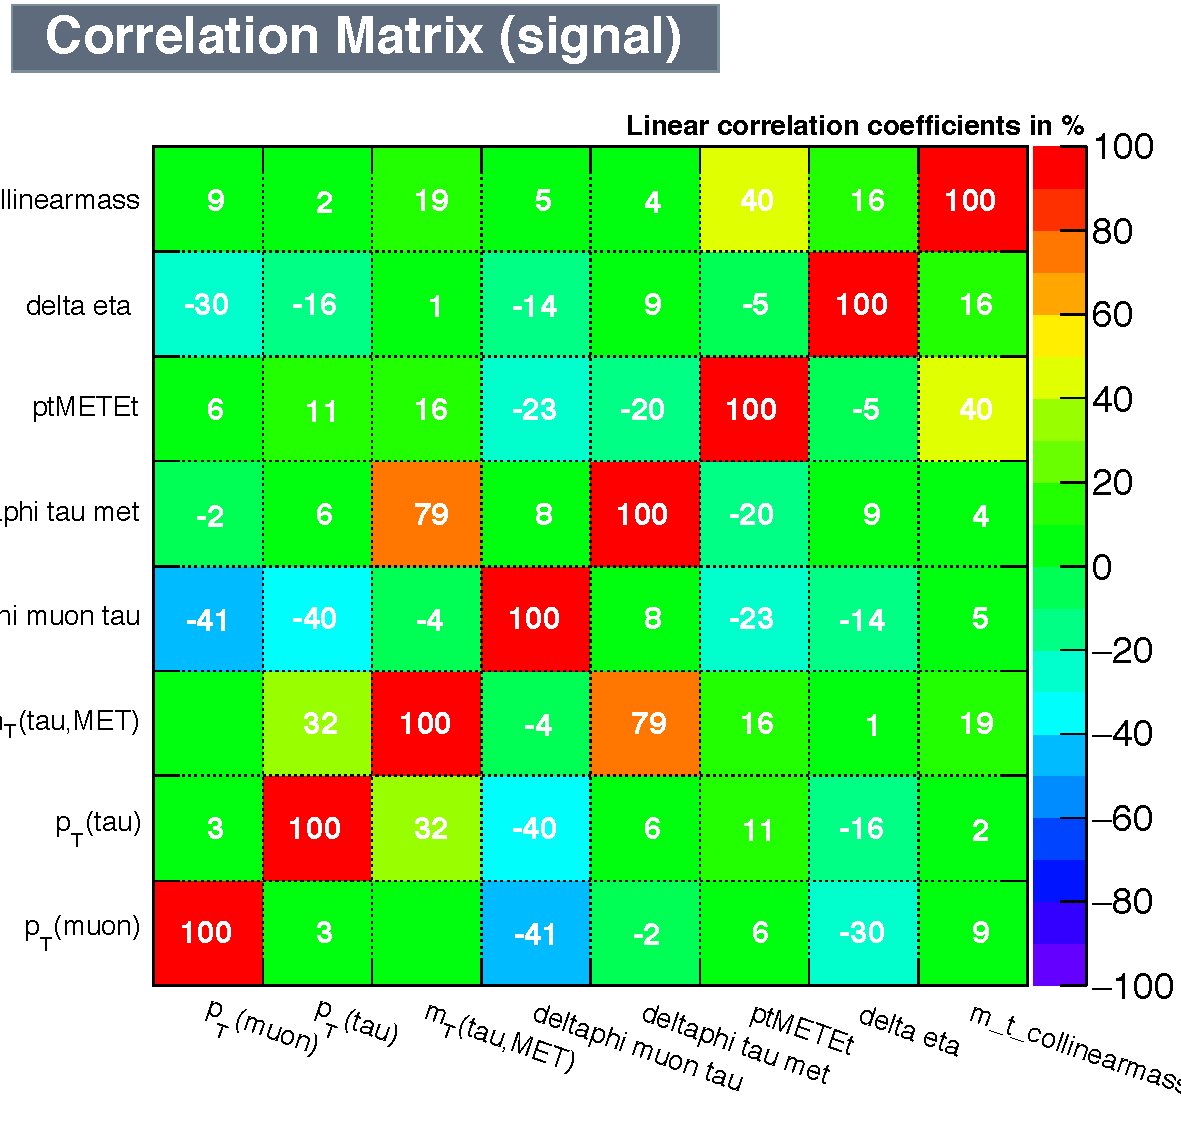
\includegraphics[width=0.4\textwidth]{chapter5/CorrelationMatrixS.pdf}}
     \subfigure[Background sample variable correlation]{ 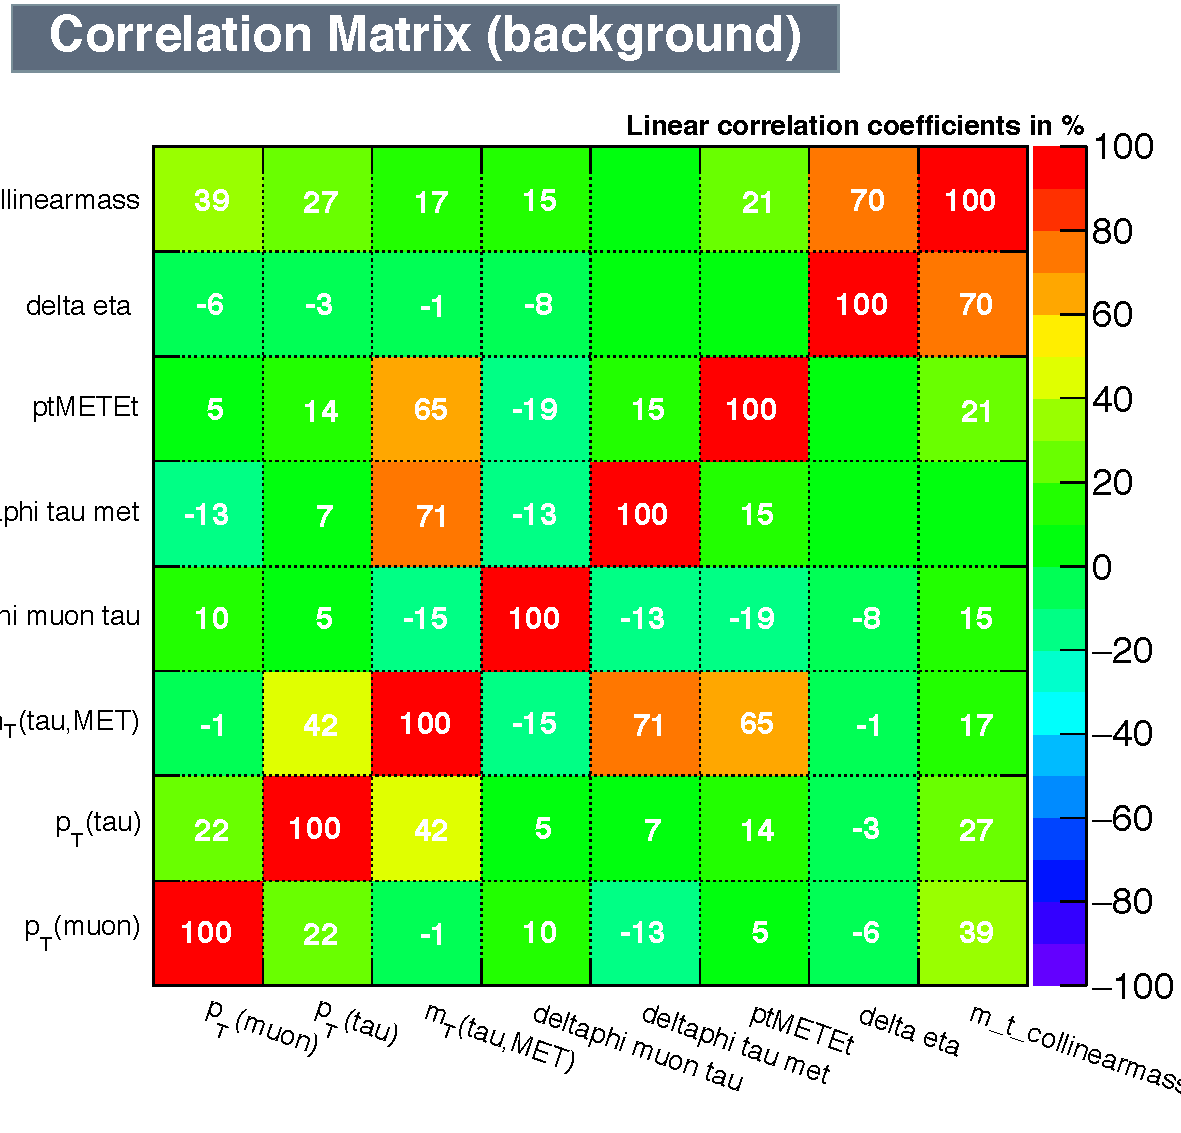
\includegraphics[width=0.4\textwidth]{chapter5/CorrelationMatrixB.pdf}}\\
     \caption{Expected limits based on an Asimov dataset as a function of $M_T(\tau, MET)$ for the different categories.}
     \label{fig:BDTvarcorrelation}
\end{figure}


The chosen input variables show low correlation in both samples as shown in Figure.~\ref{fig:BDTvarcorrelation}. In the training process, overtraining needs to be carefully treated. The overtraining problem refers to the case that the classifier between signal and background samples are specific to the particular training sample used. The training recognizes the specific features that only occurs in the training samples. Most of the time, these features are caused by the limited number of training events or with the same number of events, too many variables with weak distinguishing power are used. The TMVA overtraining checks is performed by checking with the testing samples to see if similar distinguishing power can be achieved with the output weight file from the training samples. Training and testing samples show good agreement and the training process exempts from overtraining as indicated in Figure.~\ref{fig:BDTovertraining}.
\begin{figure}[htbp] 
\centering
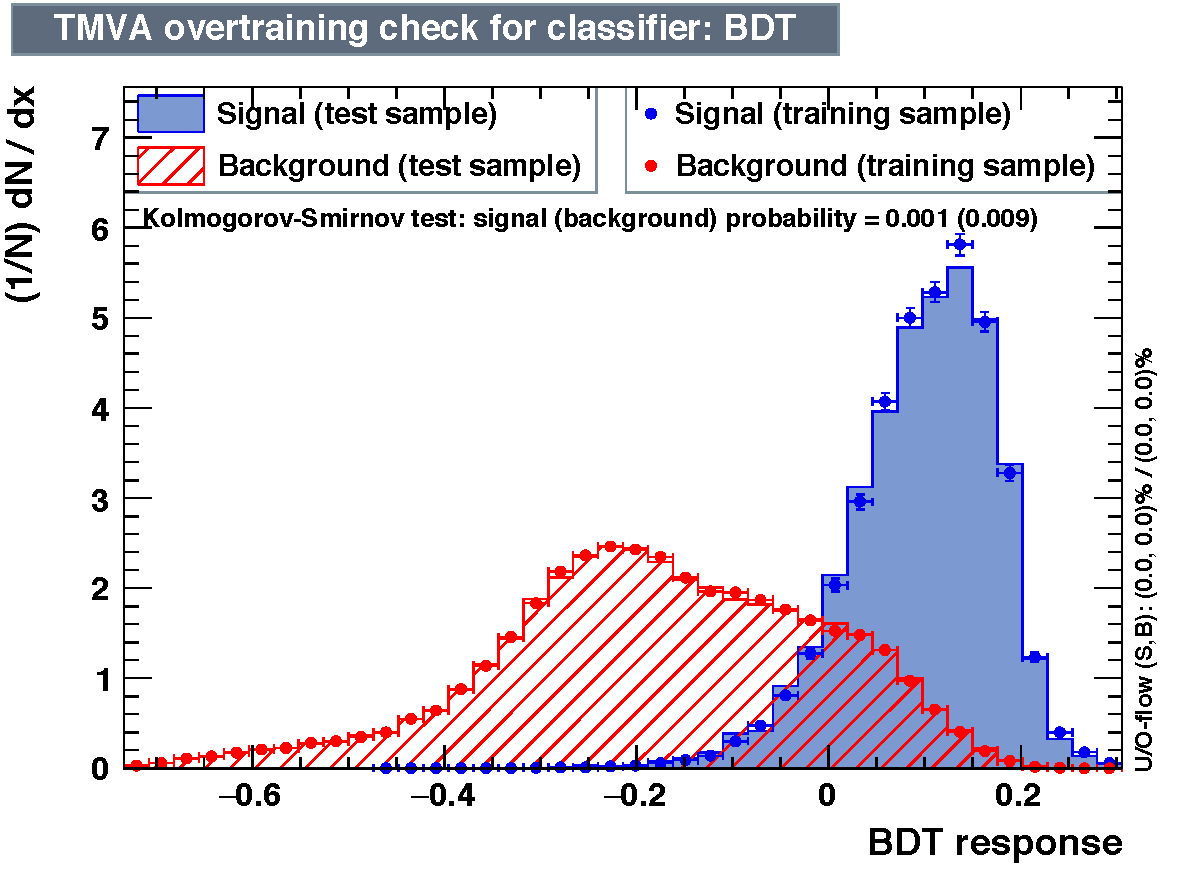
\includegraphics[width=0.6\textwidth]{chapter5/overtrain_BDT.pdf}
\caption{Overtraining checking for the BDT training in the TMVA package.}
\label{fig:BDTovertraining}
\end{figure}

\section{\texorpdfstring{$H\rightarrow e \tau_h$}{Lg}}

\subsection{Loose selection}
In $ \Hehad$ channel, trigger $HLT\_Ele27\_WP80$ is used, which applies an electron $\pt$ cut at 27 GeV at HLT level. A further cut on electron $P_{T}>30$ GeV is applied. Electrons are also required to have $|\eta_{e}<2.3|$ and $D_{z}<0.2 cm$. $D_{z}$ is the longitudinal impact parameter that shows the displacement between primary vertex and track path. Electrons are required to pass the MVA based tight ID and cut based PF tight isolation  $I_{rel}^{e}<0.1$. Tau candidates are required to have $P_{T}>30$ GeV, pseudorapidity $|\eta^{\tau}<2.3|$ and the longitudinal impact parameter $D_{z}<0.2$ cm. Tau isolation used is the cut based tight tau isolation. In addition, tau candidates are required to pass the tau Decay mode finding and tau discriminator against electrons and muons. The analysis also requires no extra isolated electrons with $\pt>10$ GeV and extra taus with $\pt>20$ GeV. Tau and electron candidates are required to have opposite sign of charges and separate with $\Delta R>0.4$ from any jets in the events with $\pt>30$ GeV. All of the requirements contribute to the selections of good qualities candidates. The datasets are binned into three categories according to the number of jets in the events:
\begin{enumerate}
\item[{\bf 0-jet:}] No events have jets pass the loose PF ID and  with jet $P_T>30$ GeV, $|\eta|<4.7$. This category enhances the gluon-gluon fusion contribution.
\item[{\bf 1-jet:}] Events with one jet passes loose PF ID and jet $P_T>30$ GeV , $|\eta|<4.7$. This category enhances the gluon-gluon fusion production with initial state radiation.
\item [{\bf 2 jets:}] Events with two jets pass loose PF ID and with jet $P_T>30$ GeV and $|\eta|<4.7$, This category contains both Higgs production mode and with an enhancement in VBF production mode. \end{enumerate}

With the preselection and binning of the jets numbers, the $\mcol$ distribution of $\Hehad$ in different categories are shown in Figure.~\ref{fig:etauCol_preselection}
\begin{figure}[hbtp]\centering
 \subfigure[0 jet]{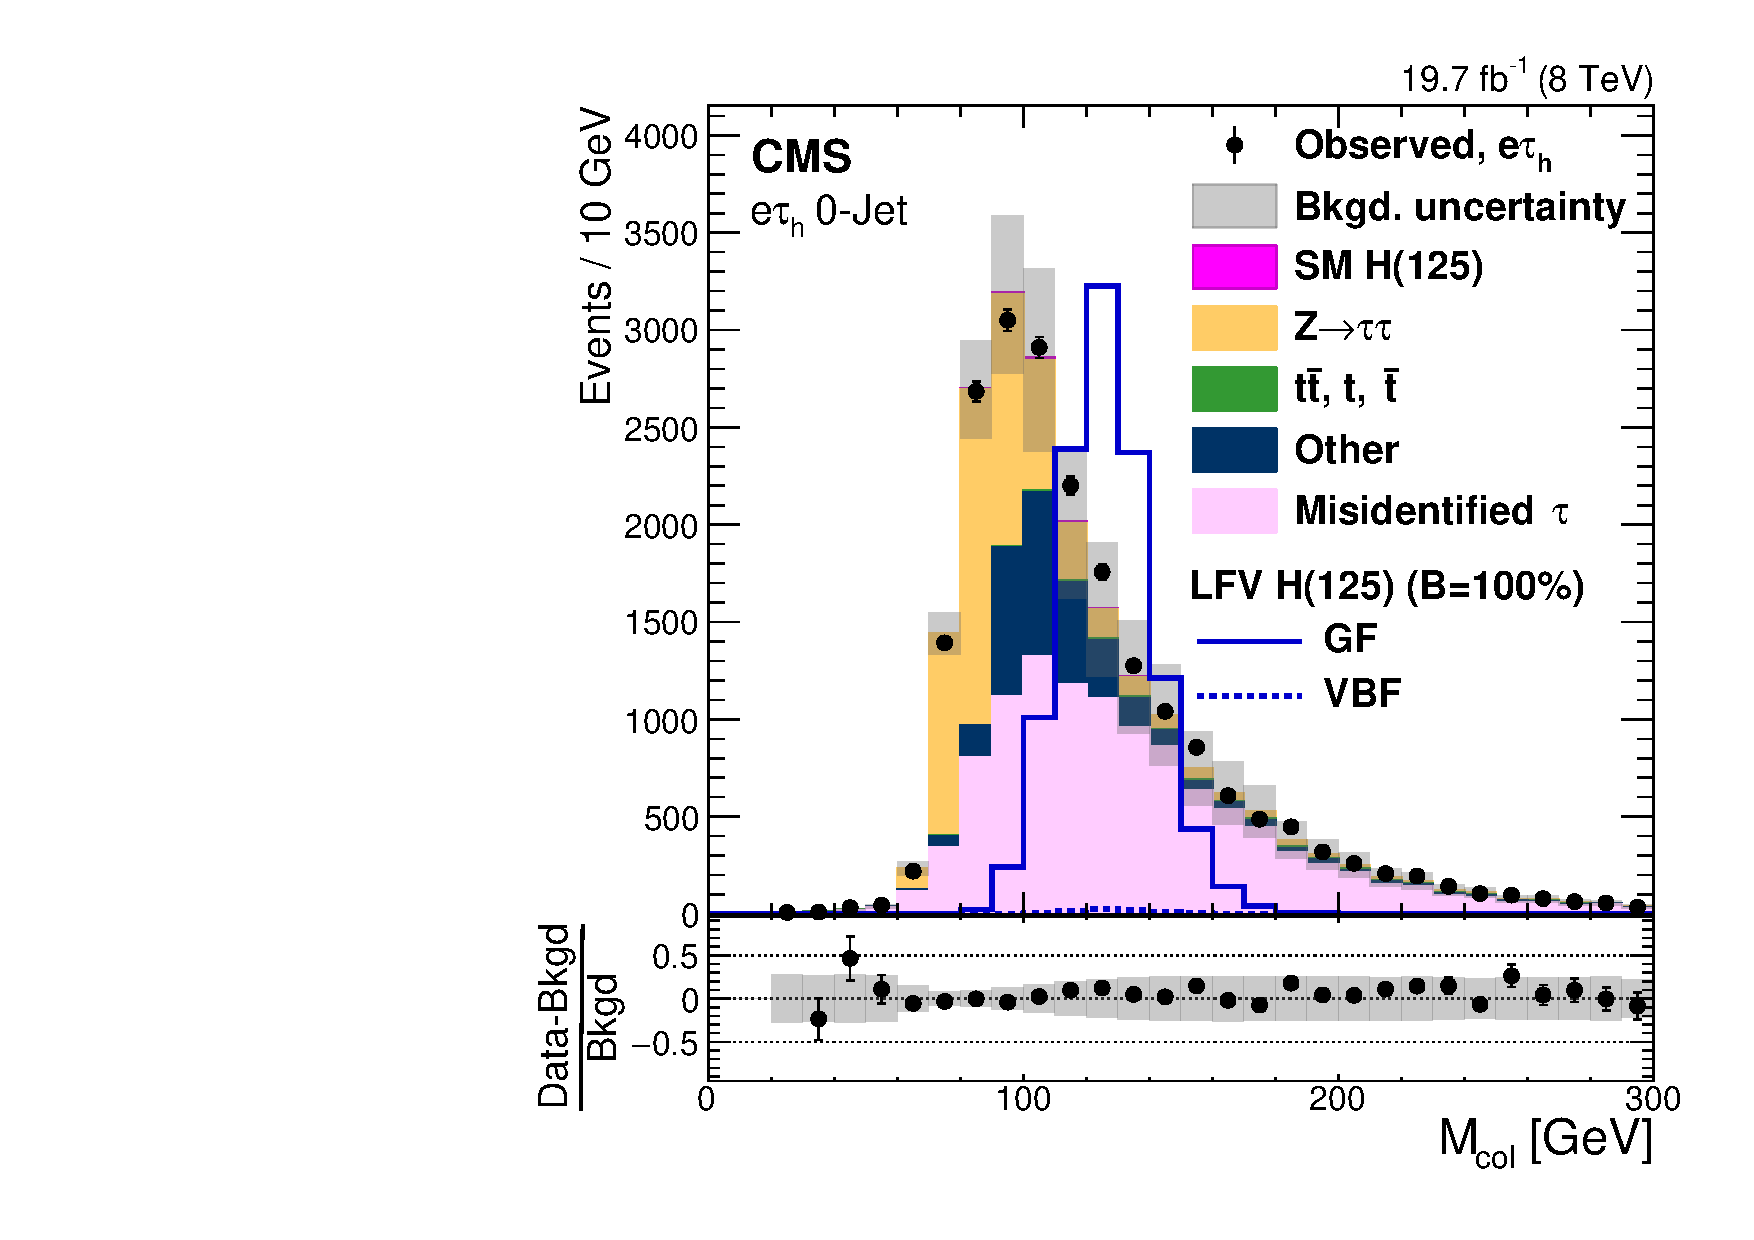
\includegraphics[width=0.4565\textwidth]{chapter5/etauPlots/etau_preselection0jet.pdf}}
 \subfigure[1 jet]{ 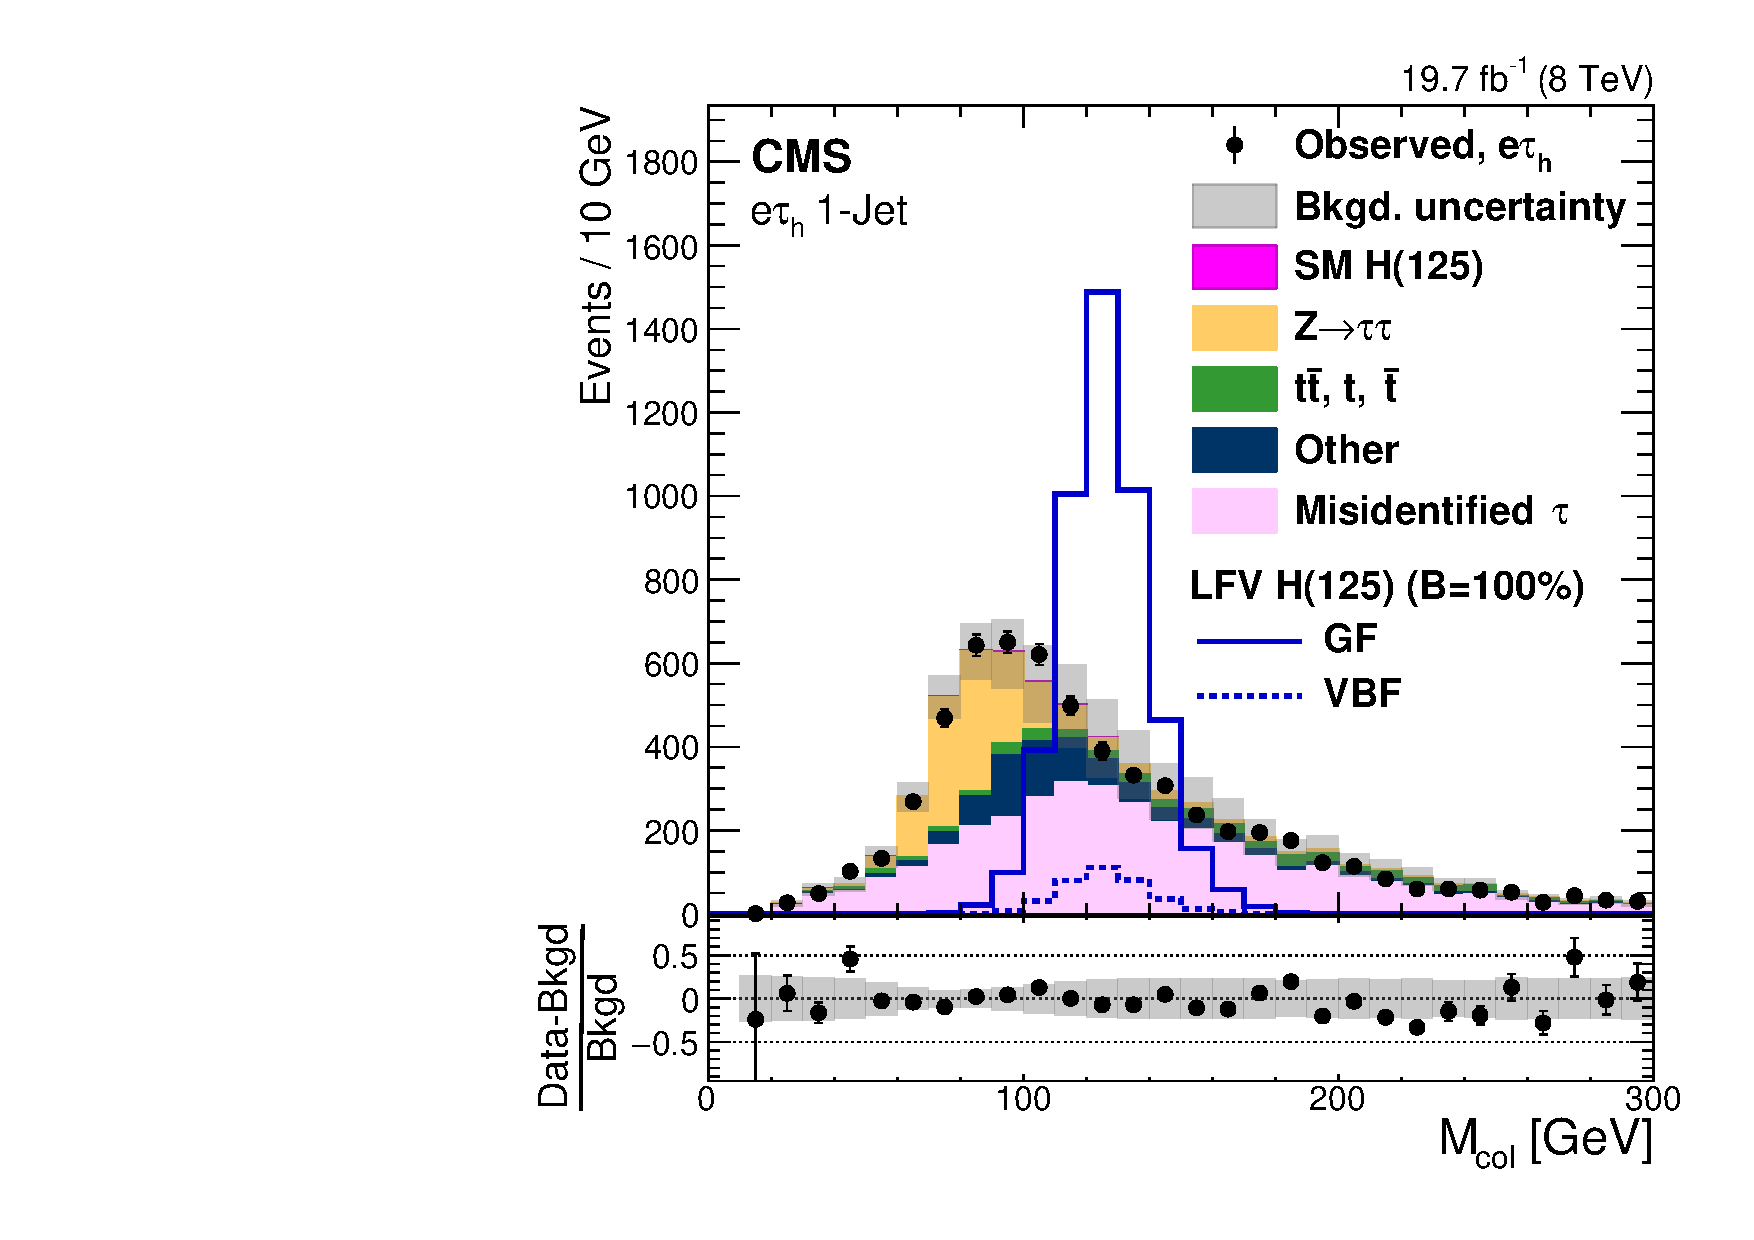
\includegraphics[width=0.4565\textwidth]{chapter5/etauPlots/etau_preselection1jet.pdf}}
 \subfigure[2 jets]{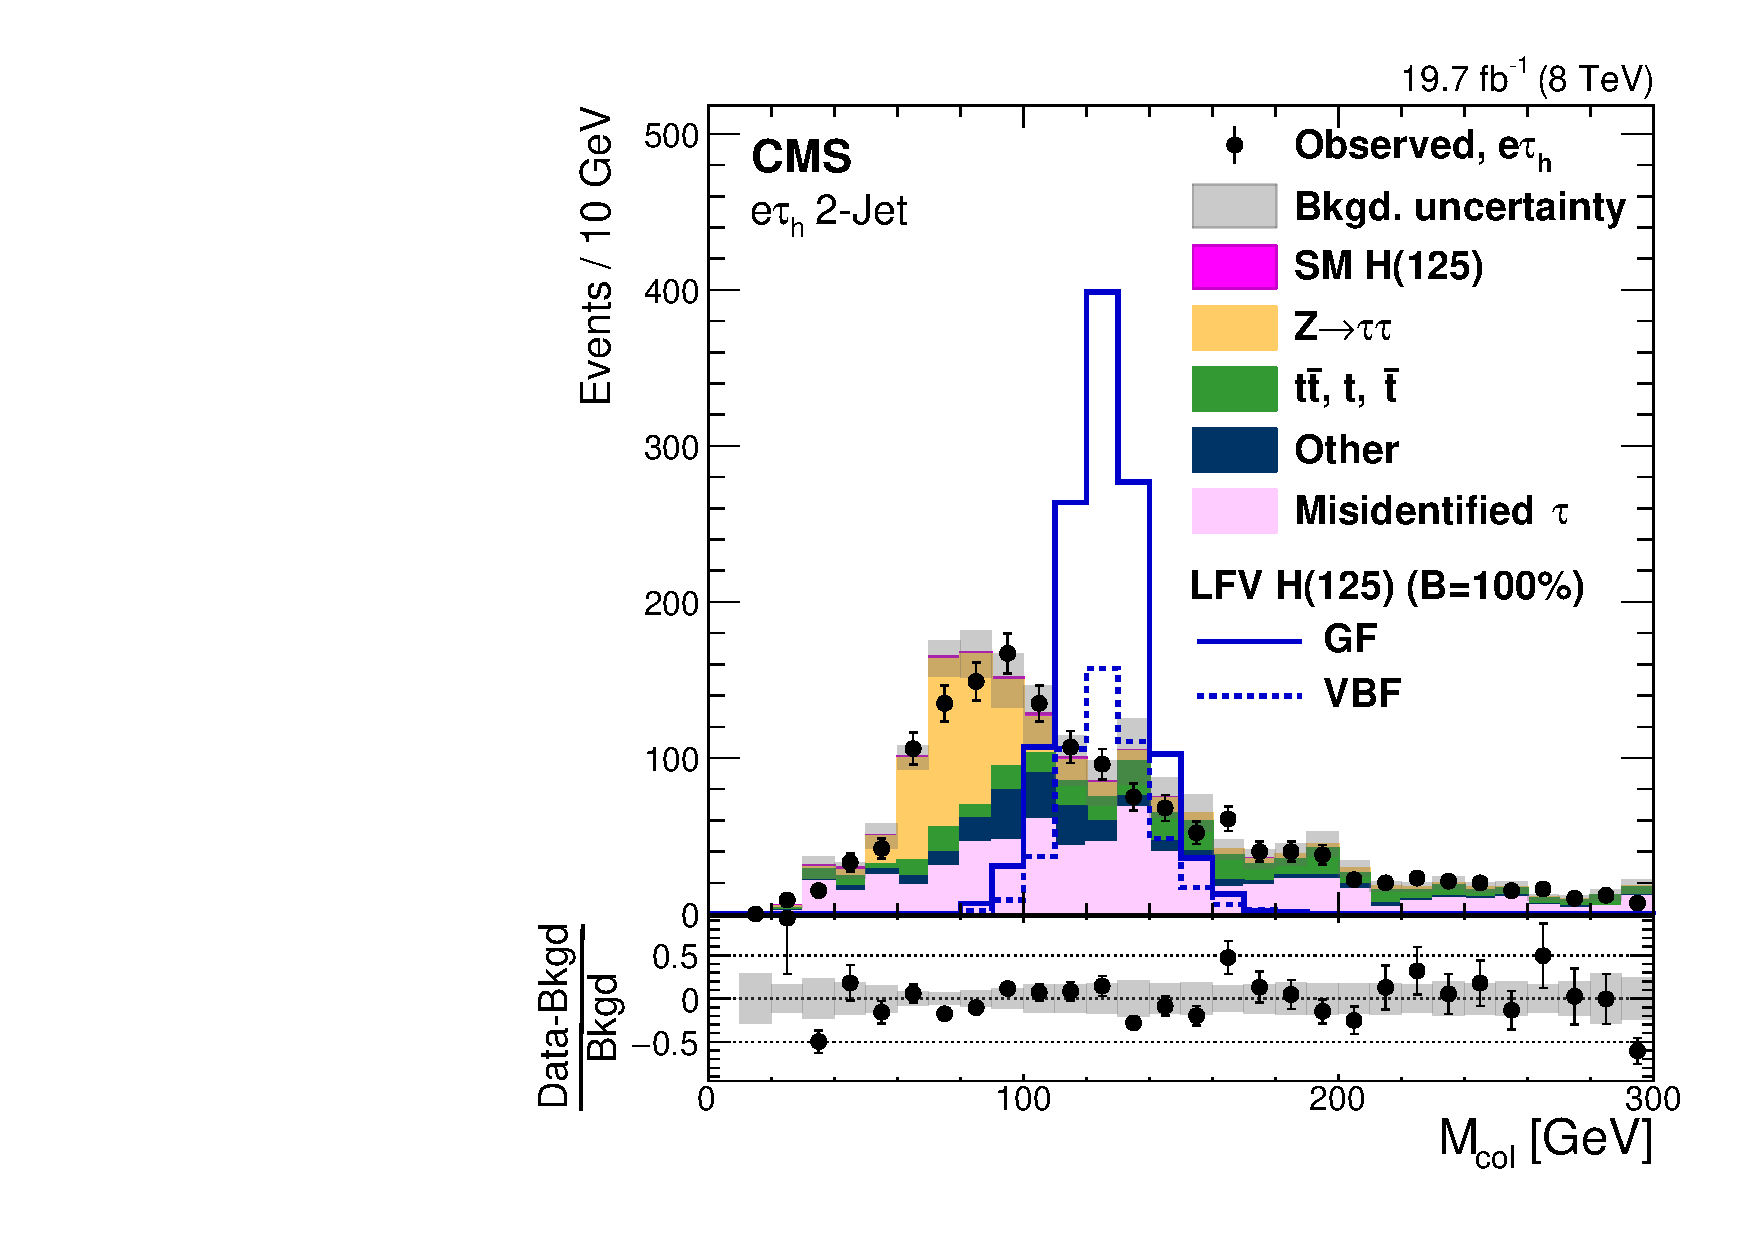
\includegraphics[width=0.4565\textwidth]{chapter5/etauPlots/etau_preselection2jet.pdf}}
 \caption{With loose selection conditions, the comparison of the observed collinear mass distributions with background from prediction. The shaded grey bands indicate the total background uncertainty.
The open histograms correspond to the expected signal distributions for $\mathcal{B}(\Hehad)=100\%$ in the  0-jet, 1-jet and 2-jet categories, respectively.}
\label{fig:etauCol_preselection}\end{figure}


\subsection{Cut-based analysis}
A set of kinematics variables are used to further select signal events. In $\Hehad$ channel, similar to the $\Hmuhad$, muon and tau leptons from the signal events are highly boosted so as $\pt$ variables play an important role in distinguishing from background events and the separation in $\phi$ direction is bigger between $\mu$ and $\tau$ of signal events. The variable $M_{T}(\tau_{h})$ which is the transverse mass form by the reconstructed $\tau$ and MET is also used in the selection. In the two jets category, the invariant mass of two jets $M_{jj}$ is used as a cut variable.  The cuts have been optimized to have the most stringent expected limits with the Asimov dataset. The detailed cuts used for $\Hehad$ is shown in table.~\ref{tab:ehadcategories}.


\begin{table}[hbtp]
  \begin{center}
  \caption{Selection criteria for each event category after cut
    optimization, for the $\Hehad$ channel}
  \begin{tabular}{l} \hline
  {\bf 0-jet category} \\ \hline
  \tabitem $\pt^{e}>45$ GeV, $\pt^{\tau}>30$ GeV, $\Delta \phi_{e \tau}>2.3$ \\
  \tabitem $M_T(\tau)<70$ GeV \\
  \tabitem No jets with $\pt^{jet}>30$ GeV, $|\eta|<4.7$, LooseID \\ \hline
 {\bf 1-jet category} \\ \hline
  \tabitem $\pt^{e}>35 $GeV, $\pt^{\tau}>40$ GeV \\
  \tabitem One jet  with $\pt^{jet}>30$ GeV, $|\eta|<4.7$, LooseID
  \\ \hline
  {\bf 2-jet category} \\ \hline
  \tabitem $\pt^{e}>35$ GeV, $\pt^{\tau}>30$ GeV \\
  \tabitem $M_T(\tau)<50$ GeV \\
      \tabitem $\pt^{jet1}>30$ GeV,$\pt^{jet2}>30$ GeV
      $|\eta_{jet1}|<4.7$,$|\eta_{jet2}|<4.7$, LooseID\\
      \tabitem $\Delta\eta(jet1,jet2)>2.3$\\
      \tabitem $M_{jj}>400$ GeV\\
      \tabitem Two jets with $\pt^{jet}>30$ GeV, $|\eta|<4.7$, LooseID \\ \hline
  \label{tab:ehadcategories}
\end{tabular}
\end{center}
\end{table}











